\section{Para-real method}
	
Parareal method is a parallel-in-time integration method which was introduced in 2001 by Lions, Maday and Turinici~\cite{partie2_ref1}. Parareal computes the numerical solution for multiple time steps in parallel and it is categorized as a parallel-across-the-steps method.

\subsection{Explanation}

We consider an initial value problem of the form \\
\begin{minipage}{\linewidth}
	\centering
	$\left\{\begin{aligned}
		X'&=f(t,X), \qquad t_0\le t\le T, \\
		X(t_0)&=X_0.
	\end{aligned}\right.$ \\
\end{minipage} \\

\subsubsection{Time decomposition}

\noindent Parareal method needs a decomposition of the time interval $[t_0,T]$ into $P$ slices $[t_j,t_{j+1}]$ with  $j\in\{0,\dots,P-1\}$, where $P$ is the number of process units. As we want to parallelize the algorithm, each time slice is assigned to one process. \\
We denote by $F$ an integrator which is of high accuracy and $G$ which is of low accuracy. Also, $F$ will be very expensive in terms of calculation but very accurate, and $G$ will be very cheap but very imprecise. We denote by $\Delta t_F$ the time step and by $\Delta t_G$ the coarse time step. \\
To have the right number of points in total (i.e. the sum of the number of points of each interval is equal to the number of points between $t_0$ and $T$), we are not going to cut the interval in equal parts. However, the $t_j$ will have to be multiples of $\Delta t_G$ and the final point of the fine integrator on each process should be equal to the final point of the coarse integrator. \\
To do this, let's do the following:
\begin{enumerate}[label=\textbullet]
	\item We compute the number of coarse time steps $n_G$ and the number of fine time steps $n_F$ between $t_0$ and $T$ as well as the ratio between the two $r=n_F/n_G$.
	\item We do the Euclidean division of $nb_G$ by the number of processes $P$, which gives us the number of coarse time steps on each subinterval. Then we distribute equally to each process the rest of the division.
	\item We compute the number of fine time steps on each sub-interval using $r$ such that the final time of the fine integrator and the final time of the coarse integrator are the same on each sub-interval.
	\item We then compute the $t_j$, i.e. the initial times of each subinterval, from the number of coarse time steps per process.
\end{enumerate}
For example, taking $P=3$ processes and the following parameters :
$$\Delta t_G=0.1, \quad \Delta t_F=0.01, \quad t_0=0, \quad T=10$$ 
We have :
$$n_G=100, n_F=1000, r=1000/100=10$$
Thus we can calculate the number of coarse time steps per subinterval :
$$tab_G = [34,33,33]$$
Multiplying by $r$, we obtain the number of fine time steps per subinterval :
$$tab_G = [340,330,330]$$
And we deduce the following $t_j$ :
$$times = [0,3.4,6.7,10]$$

\subsubsection{Principle of parareal method}
\label{section parareal method}

\noindent We denote by $U_j^k$, $j\in\{0,\dots,P\}$ the initial point at time $t_j$ and at iteration $k$. We also denote $F(U_{j-1}^k)$, $j\in\{1,\dots,P\}$ the result of the fine integrator between $t_{j-1}$ and $t_j$ which starts from the initial point $U_{j-1}^k$ at iteration $k$ and respectively $G(U_{j-1}^k)$, $j\in\{1,\dots,P\}$ the result of the coarse integrator between $t_{j-1}$ and $t_j$ which starts from the initial point $U_{j-1}^k$ at iteration $k$. Then, a series of steps (\textit{see Figure \ref{parareal}}) is performed until the solution of the system converges. \\

\noindent At iteration $k=0$ :
\begin{enumerate}[label=\textbullet]	
	\item Step 1 (\textit{see \ref{parareal:1}}) : At iteration $k=0$, we have an initial point $U_0^0=X_0$.
	\item Step 2 (\textit{see \ref{parareal:2}}) : We start by applying the function $G$ on all intervals $[t_j,t_{j+1}]$ and we denote by $U_j^0=G(U_{j-1}^0)$ the values of $G$ at $t_j$. \\
	Note that this part of the method must be done sequentially because if we parallelize the task, the process $j$ should wait until the process $j-1$ has finished before starting.
	\item Step 3 (\textit{see \ref{parareal:3}}) : We can then calculate from each $U_j^0$ the fine solution between $t_j$ and $t_{j+1}$ : $F(U_j^0)$. This is an operation that must be parallelized.
\end{enumerate}

\noindent At iteration $k=1$ :
\begin{enumerate}[label=\textbullet]	
	\item Step 4 (\textit{see \ref{parareal:4}}) : We can then continue to iteration $k=1$ where we need the values $G(U_j^0)$ and $F(U_j^0)$ calculated at the previous iteration ($k=0$). \\
	We will also keep the initial point at time $t_0$ : $U_0^1=U_0^0$.
	\item Step 5 (\textit{see \ref{parareal:5}}) : We can then calculate $G(U_0^1)$ which allows us to obtain the point $U_1^1$ by the following formula:
	$$U_j^1=G(U_{j-1}^1)+(F(U_{j-1}^0)-G(U_{j-1}^0)).$$
	Note that due to $U_0^1=U_0^0$, we have $G(U_0^1)=G(U_0^0)$ and therefore $U_1^1=F(U_0^0)$ \\
	We then compute in the same way the following $G(U_j^1)$ and the associated $U_{j+1}^1$ points. This step can be done sequentially for the same reason as in step 2.
	\item Step 6 (\textit{see \ref{parareal:6}}) : We can then calculate from each $U_j^1$ the fine solution between $t_j$ and $t_{j+1}$ : $F(U_j^1)$. This is an operation that must be parallelized. \\
	Note that due to $U_0^1=U_0^0$, we also have $F(U_0^1)=F(U_0^0)$.
\end{enumerate}

\noindent Then we repeat steps 3 to 6 until $U_j^k-U_j^{k-1}\rightarrow 0 \quad \forall j\in\{0,\dots,P-1\}$. \\
We have at iteration $k$:
$$U_j^k=G(U_{j-1}^k)+(F(U_{j-1}^{k-1})-G(U_{j-1}^{k-1}))$$

\noindent The following figure (Figure \ref{parareal}) illustrates the previous steps :

\begin{figure}[h]
	\captionsubfigure
	\fbox{
		\centering \qquad
		\begin{minipage}[c]{\linewidth}
			\begin{subfigure}[t]{.30\linewidth}       
				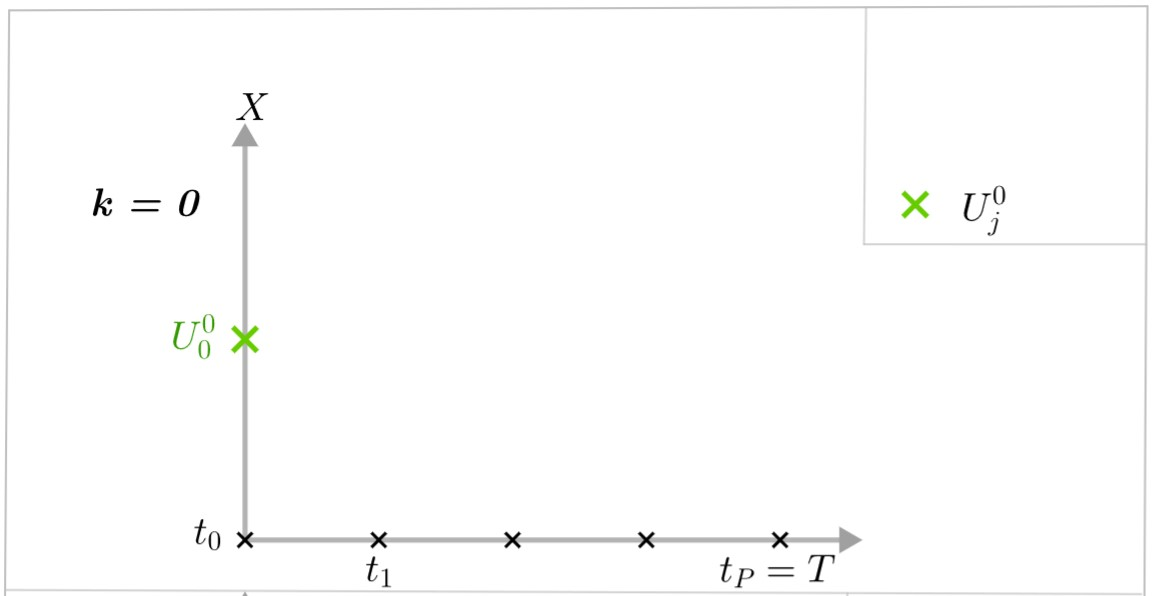
\includegraphics[width=\linewidth]{"images/parareal/explanation/parareal_1.jpg"}
				\captionof{figure}{ : Step 1}
				\label{parareal:1}
			\end{subfigure} 
			\begin{subfigure}[t]{.30\linewidth}       
				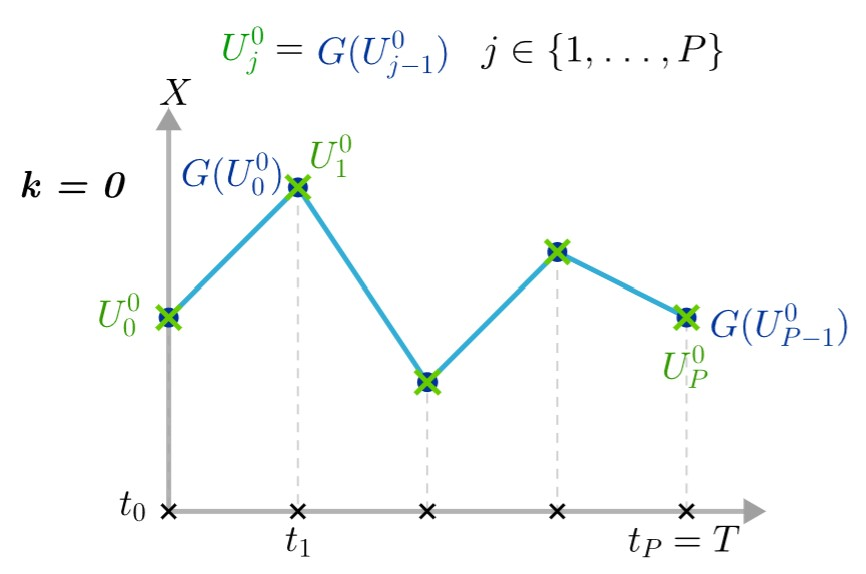
\includegraphics[width=\linewidth]{"images/parareal/explanation/parareal_2.jpg"}
				\captionof{figure}{ : Step 2}
				\label{parareal:2}
			\end{subfigure} 
			\begin{subfigure}[t]{.30\linewidth}       
				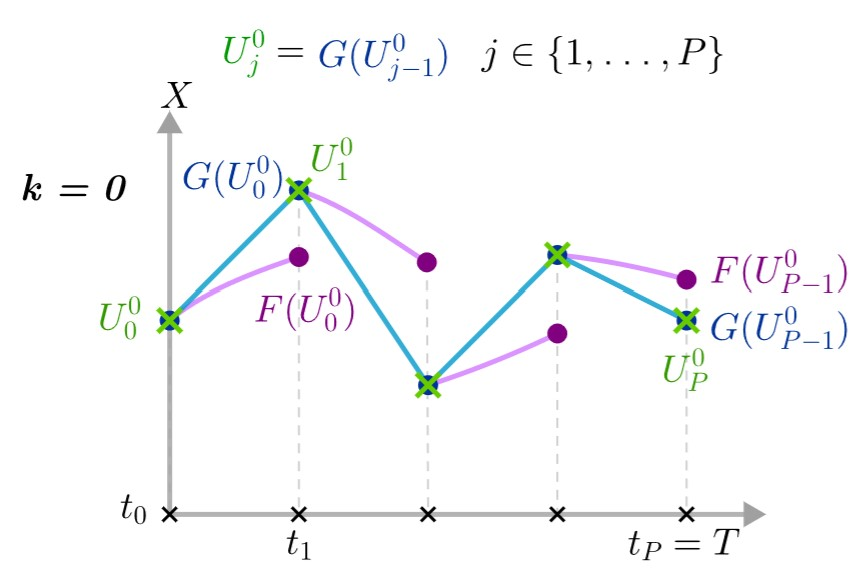
\includegraphics[width=\linewidth]{"images/parareal/explanation/parareal_3.jpg"}
				\captionof{figure}{ : Step 3}
				\label{parareal:3}
			\end{subfigure} 
			
			\begin{subfigure}[t]{.30\linewidth}       
				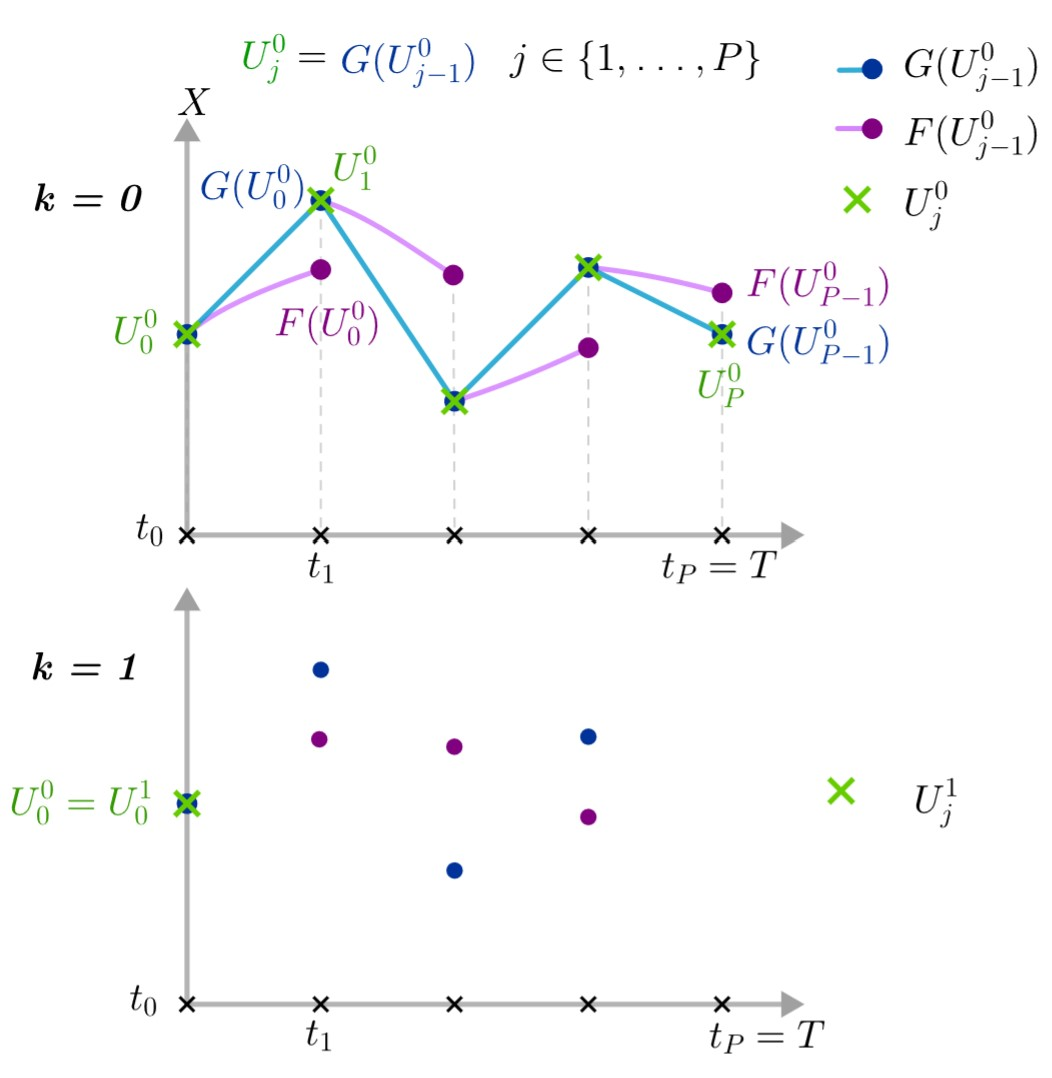
\includegraphics[width=\linewidth]{"images/parareal/explanation/parareal_4.jpg"}
				\captionof{figure}{ : Step 4}
				\label{parareal:4}
			\end{subfigure} 
			\begin{subfigure}[t]{.30\linewidth}  
				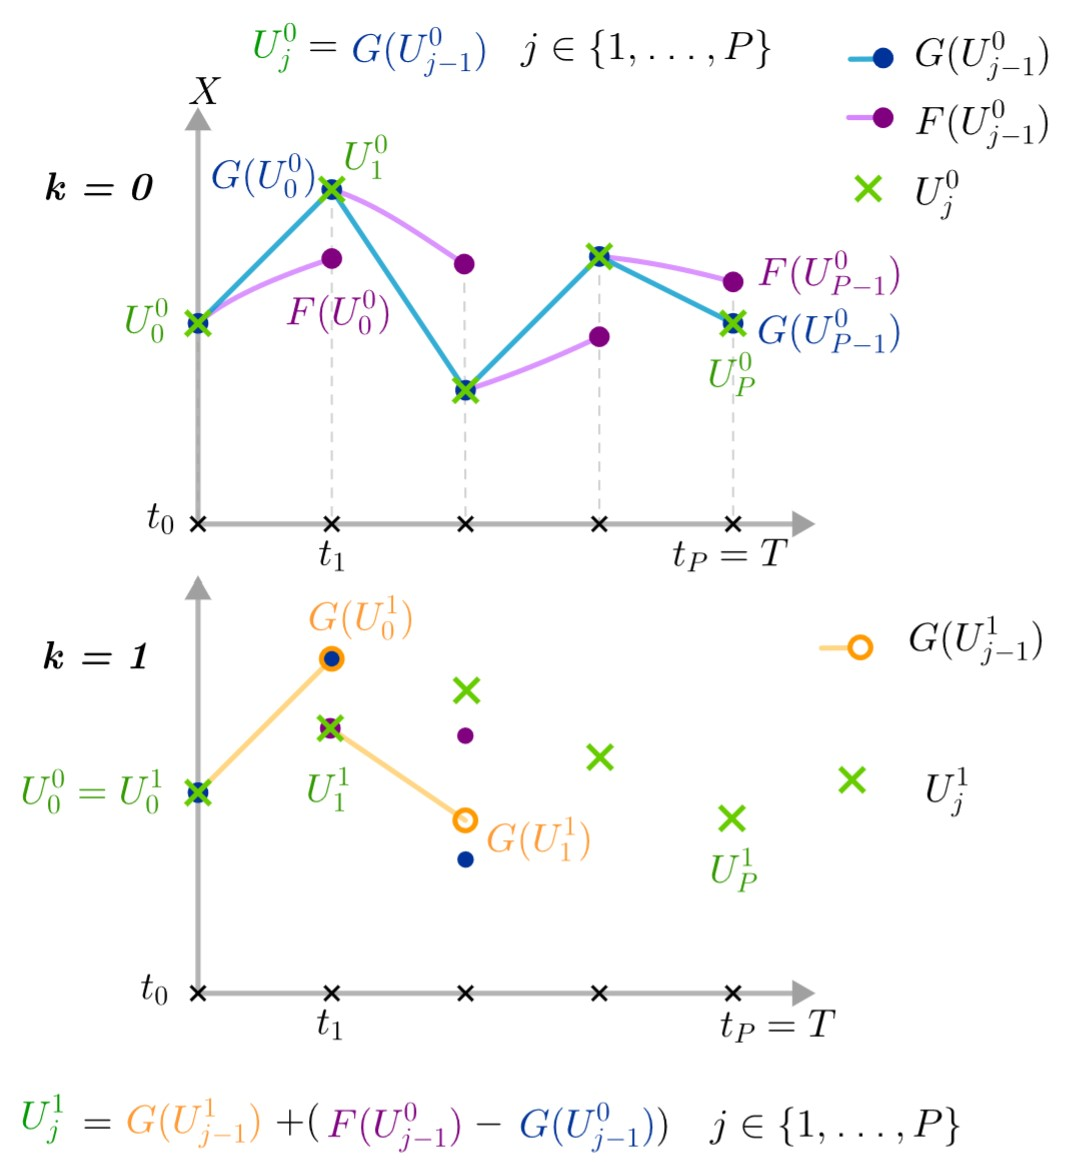
\includegraphics[width=\linewidth]{"images/parareal/explanation/parareal_5.jpg"}
				\captionof{figure}{ : Step 5}
				\label{parareal:5}
			\end{subfigure} 
			\begin{subfigure}[t]{.30\linewidth}      
				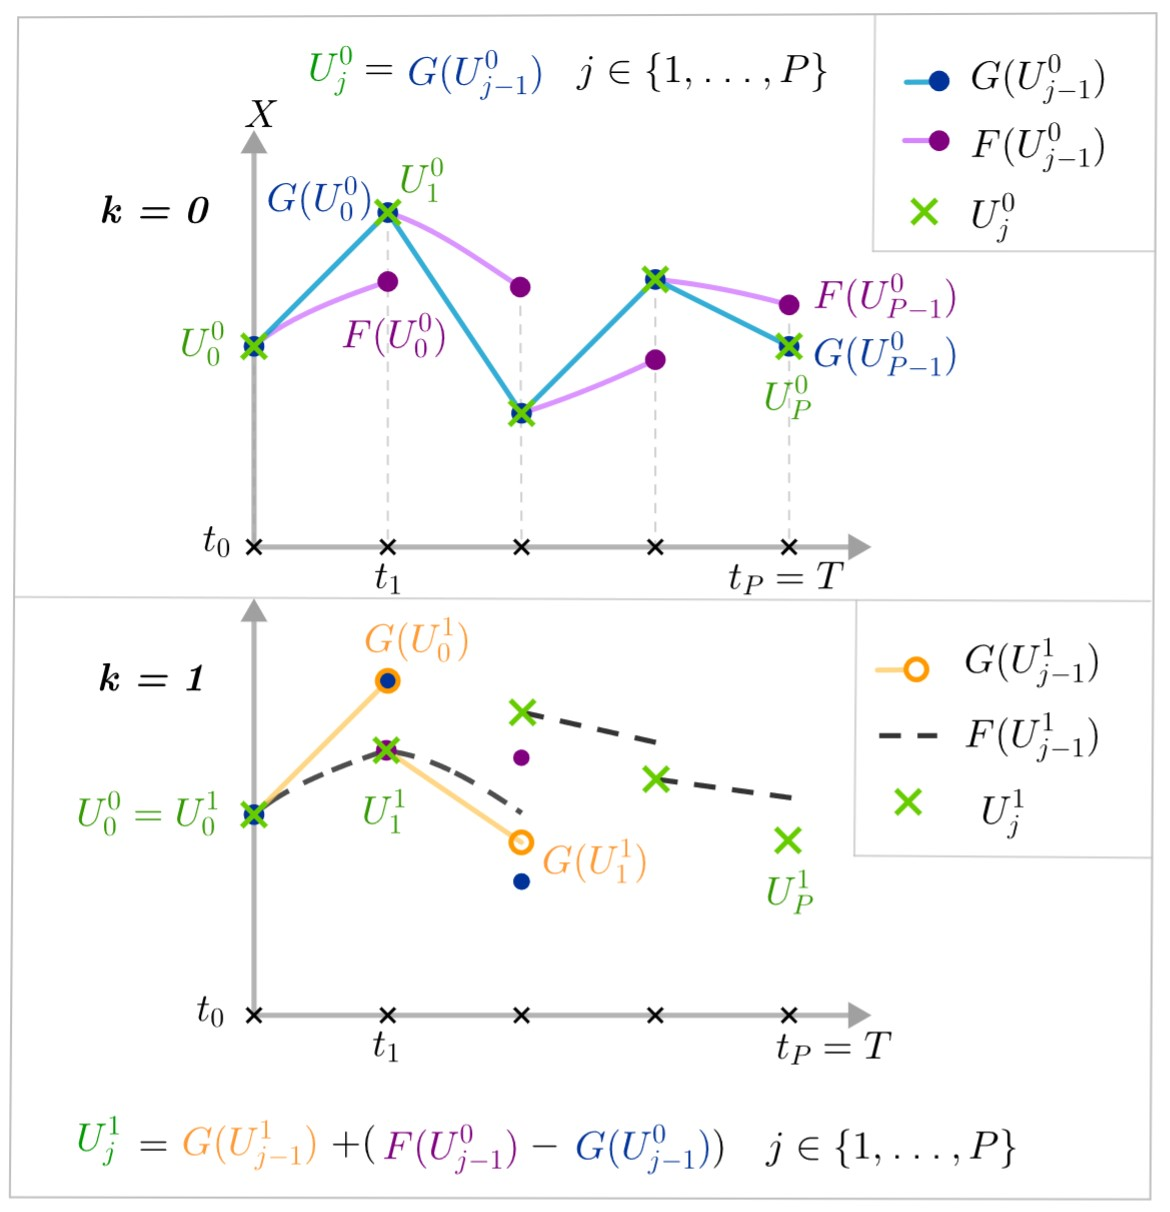
\includegraphics[width=\linewidth]{"images/parareal/explanation/parareal_6.jpg"}
				\captionof{figure}{ : Step 6}
				\label{parareal:6}
			\end{subfigure}
	\end{minipage}}
	\caption{Parareal method}
	\label{parareal}
\end{figure}


\noindent \underline{\textit{Remarks :}} At iteration k.
\begin{itemize}[label=-]
	\item We have : $\qquad U_0^k=U_0^0=X_0 \quad \forall k$.
	\item Note that the first 2 steps are always done because there can't be convergence with only one value. So, for example, if we take only one process and we apply the parareal method, we will have at the first iteration ($k=0$) only one initial point $U_0^0=X_0$ and we will compute the fine and coarse solution only on this point. We can then go to the next iteration, which will be exactly the same, and the algorithm will stop immediately. Indeed, there will be convergence between $U_0^0$ and $U_0^1$ (because they are equal), moreover there is obviously convergence between the 2 solutions. However, there is still one extra iteration ($k=1$) and the computation of the coarse solution is also useless because it is not used to update the other initial points due to the fact that there is only one.
	\item We can also notice that the calculations which are done on the last interval $[t_{P-1},t_P]$ are not used because the points $U_P^k$ are not useful for the method. On this interval, one could then compute the fine solution only if there is convergence.
\end{itemize}

\subsubsection{Algorithm}

\fbox{TO COMPLETE !!!!!}

\subsubsection{Order of parareal method}
\label{order}

We say that the previous method is of order k (see \cite{partie2_ref2}) if there is a constant $c_k$ such that :
\begin{equation}
	\forall j\in\{0,\dots,P-1\} \qquad |U_j^k-U_{ex}(t_j)|+\max_{t\in[t_j,t_{j+1}]}|U_k(t)-U_{ex}(t)|\le c_k(\Delta t_G)^k
\end{equation}
where $U_j^k$ is the initial point at $t_j$ and iteration $k$, $U_{ex}(t_j)$ is the exact solution at the same time (at $t_j$ and iteration $k$), $U_k$ is the solution between $t_0$ and $T$ at iteration k and $U_{ex}$ is the exact solution between $t_0$ and $T$. Note that we calculate the maximum just between $t_j$ and $t_{j+1}$. \\

\noindent In the following, we will note : $$\mathcal{E}(j,k)=|U_j^k-U_{ex}(t_j)|+\max_{t\in[t_j,t_{j+1}]}|U_k(t)-U_{ex}(t)|$$



\newpage

\subsection{Application in Python and C++}

During the project, we have already implemented the parareal method in Python and obtained some results that will be presented in this section. One of the objectives of the internship was to implement it in C++ using MPI. In this section, as for the project, we will only focus on the following ODEs : Harmonic oscillator (see Section \ref{oscillator_ode}) and Lorenz system (see Section \ref{lorenz_ode}).

\subsubsection{Results}

After implementing the parareal method in C++ and Python we saved the results at each iteration in csv files to see the results. For the results of the parareal method implemented in Python as for the one implemented in C++, the reading of the csv files and the display of the results is done with Python. \\
For the two integrators of the Parareal method, we will take Runge Kutta order 4 method (see Section \ref{rk4}) with a small time step for $F$ and a larger one for $G$. 

\begin{enumerate}[label=\textbullet]
	\item \textbf{Harmonic oscillator :} \\
	We want to apply the parareal method on the harmonic oscillator. With the previous example of the Section \ref{oscillator_ode}, we have the following parameters with 3 process :
	$$x(0)=0,\quad v(0)=1, \quad\omega_0=5, \quad x_0=\frac{-1}{5}, \quad \phi_0=\frac{\pi}{2}$$
	We then obtain the following result with the parareal method in Python according to the iterations of the method :
	\begin{figure}[H]
		\centering
		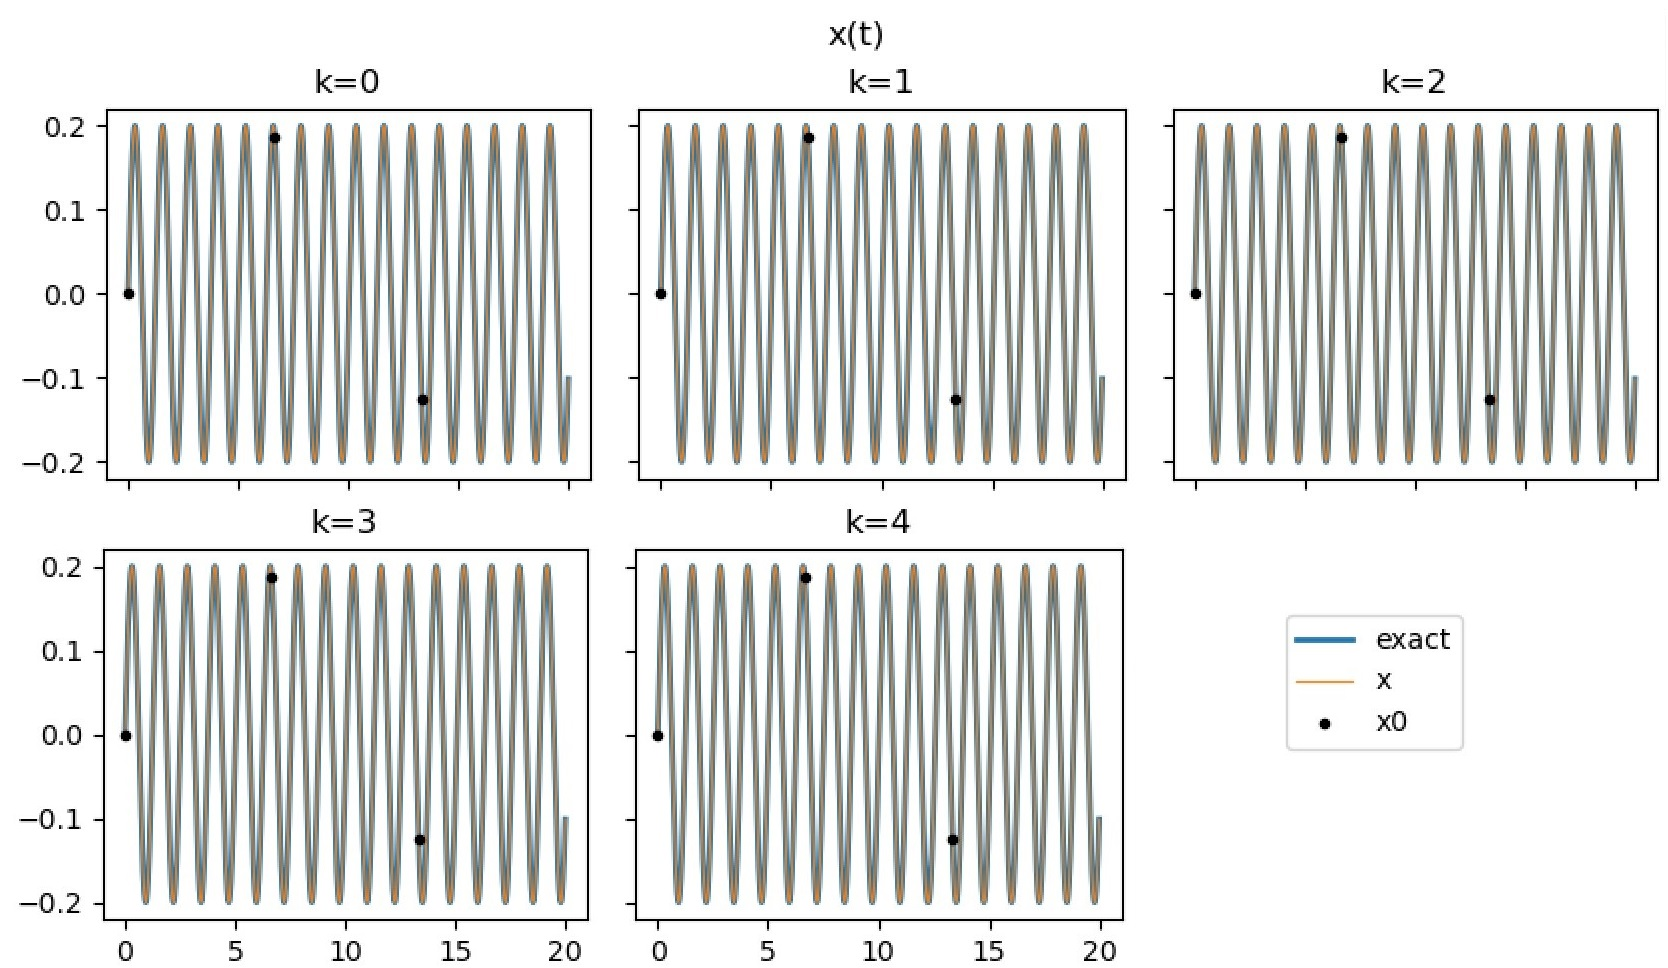
\includegraphics[width=0.7\linewidth]{"images/parareal/cpp/osci_1.jpg"}
		\caption{Exact solution vs Approximate solution for given parameters (in \textbf{Python})}
	\end{figure}
	\noindent We see that the system seems to converge in 5 iterations, i.e. between the iterations $k=4$ and $k=5$ the points $U_n^k$ are equal to almost one $\epsilon$. 
	
	\item \textbf{Lorenz system :} \\
	
	We choose the following parameters :
	$$\sigma=10, \quad b=\frac{8}{3}, \quad r=28, \quad X_0=(5,5,5)$$
	$$t_0=0, \quad T=20, \quad P=4,\quad \Delta t_G=0.1, \quad \Delta t_F=0.01$$
	For this choice of parameters, we have a butterfly wing pattern (see Figure \ref{lorenz:exact3D}) and we have the three following curves (see Figure \ref{lorenz:exact}) for the representation of the 3 variables x, y and z as functions of time.
	\begin{figure}[H]       
		\begin{minipage}[t]{0.48\linewidth}
			\centering
			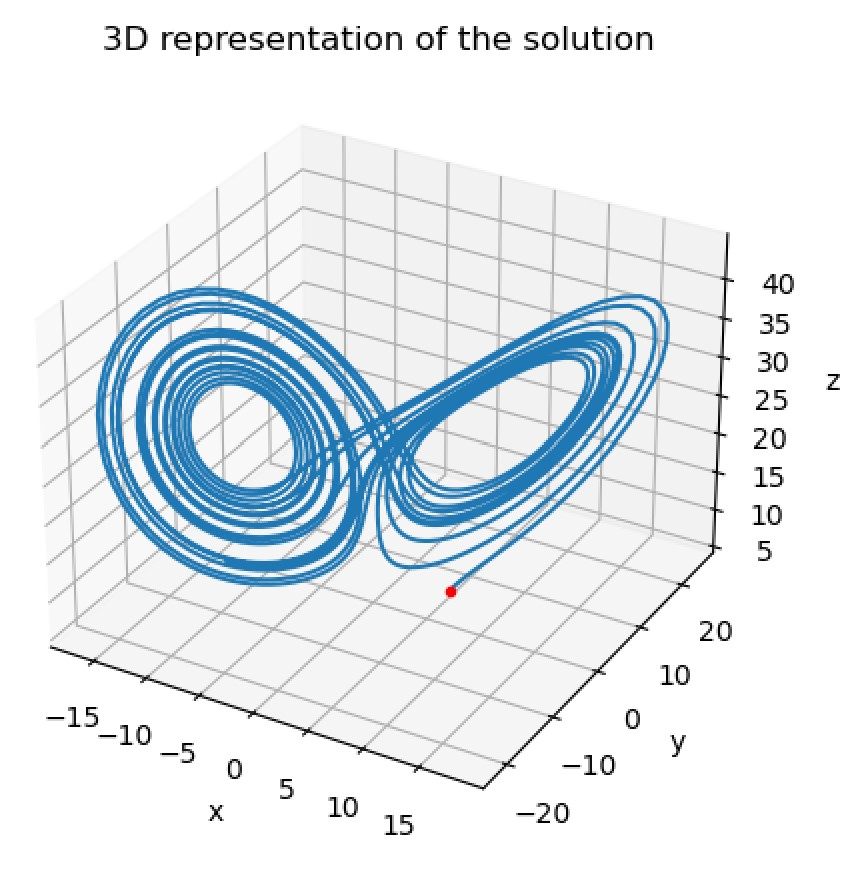
\includegraphics[width=0.9\linewidth]{"images/parareal/cpp/lorenz_exact_3D.jpg"}
		\end{minipage} \hfill
		\begin{minipage}[t]{0.48\linewidth}
			\centering
			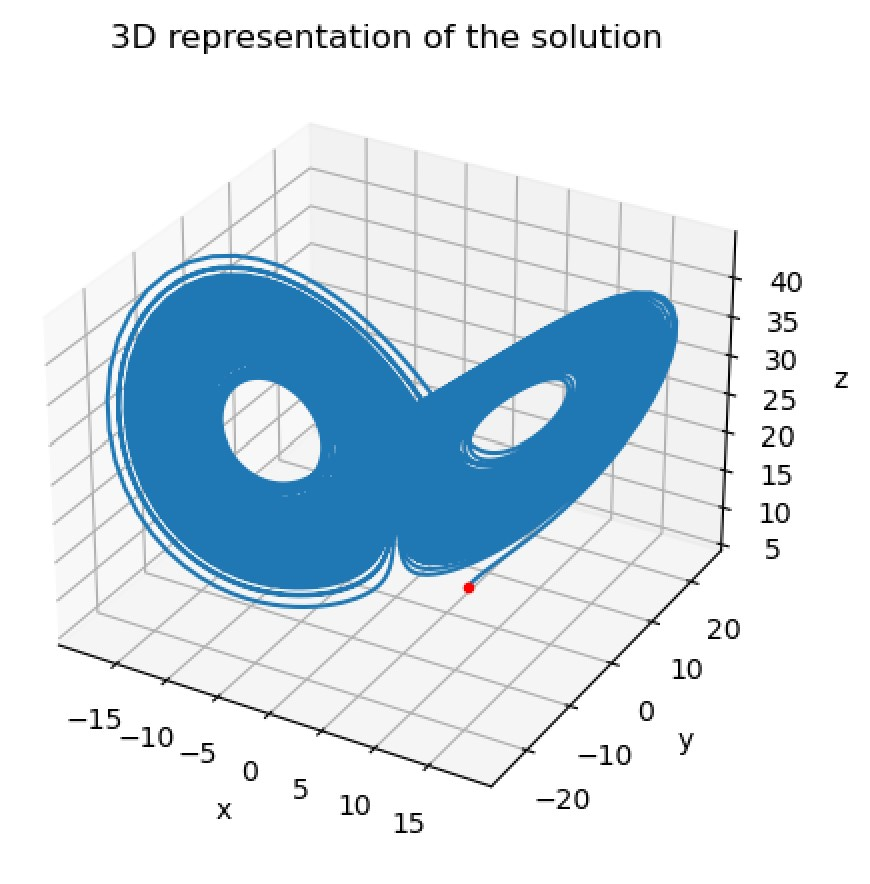
\includegraphics[width=0.9\linewidth]{"images/parareal/cpp/lorenz_exact_3D_T200.jpg"}
		\end{minipage}
		\captionof{figure}{Solution 3D of the Lorenz system with given parameters ($T=20$ and $T=200$)}
		\label{lorenz:exact3D}
	\end{figure}
	\begin{figure}[H]  
		\centering     
		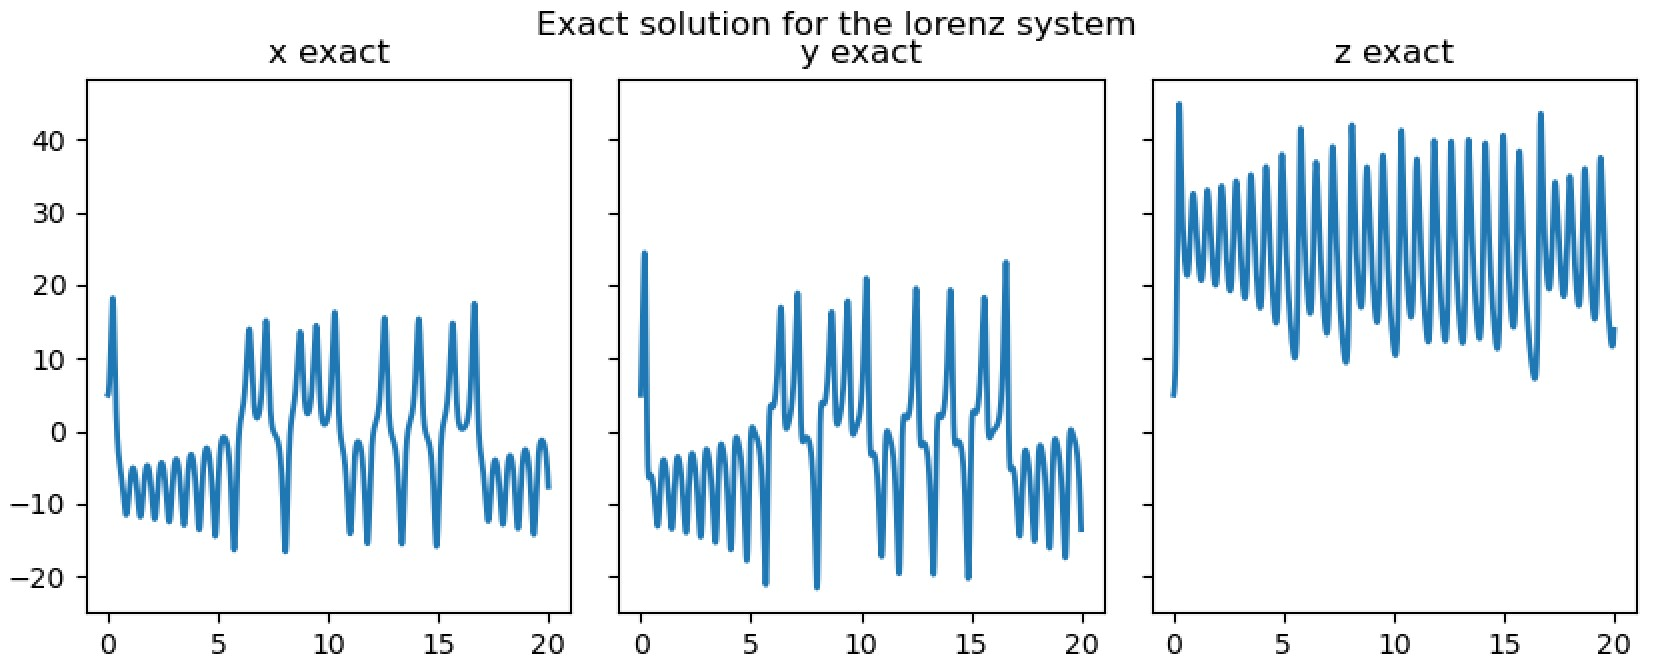
\includegraphics[width=0.9\linewidth]{"images/parareal/cpp/lorenz_exact.jpg"}
		\captionof{figure}{Solution of the Lorenz system with given parameters}
		\label{lorenz:exact}
	\end{figure}

	We will now apply the parareal method in \textbf{C++} with the previous parameters for different numbers of processes (from 1 to 4 processes : see Figures \ref{lorenz:1}, \ref{lorenz:2}, \ref{lorenz:3} and \ref{lorenz:4}). We are going to be interested here only in the variable x.

	\begin{enumerate}[label=-]
	
		\item With 1 process we see (as explained in the "Remarks" of the section \ref{section parareal method}) that there are only two iterations and that they are similar (because they start from the same initial point and there is no other initial point).
		\begin{figure}[H]       
			\qquad \qquad \qquad 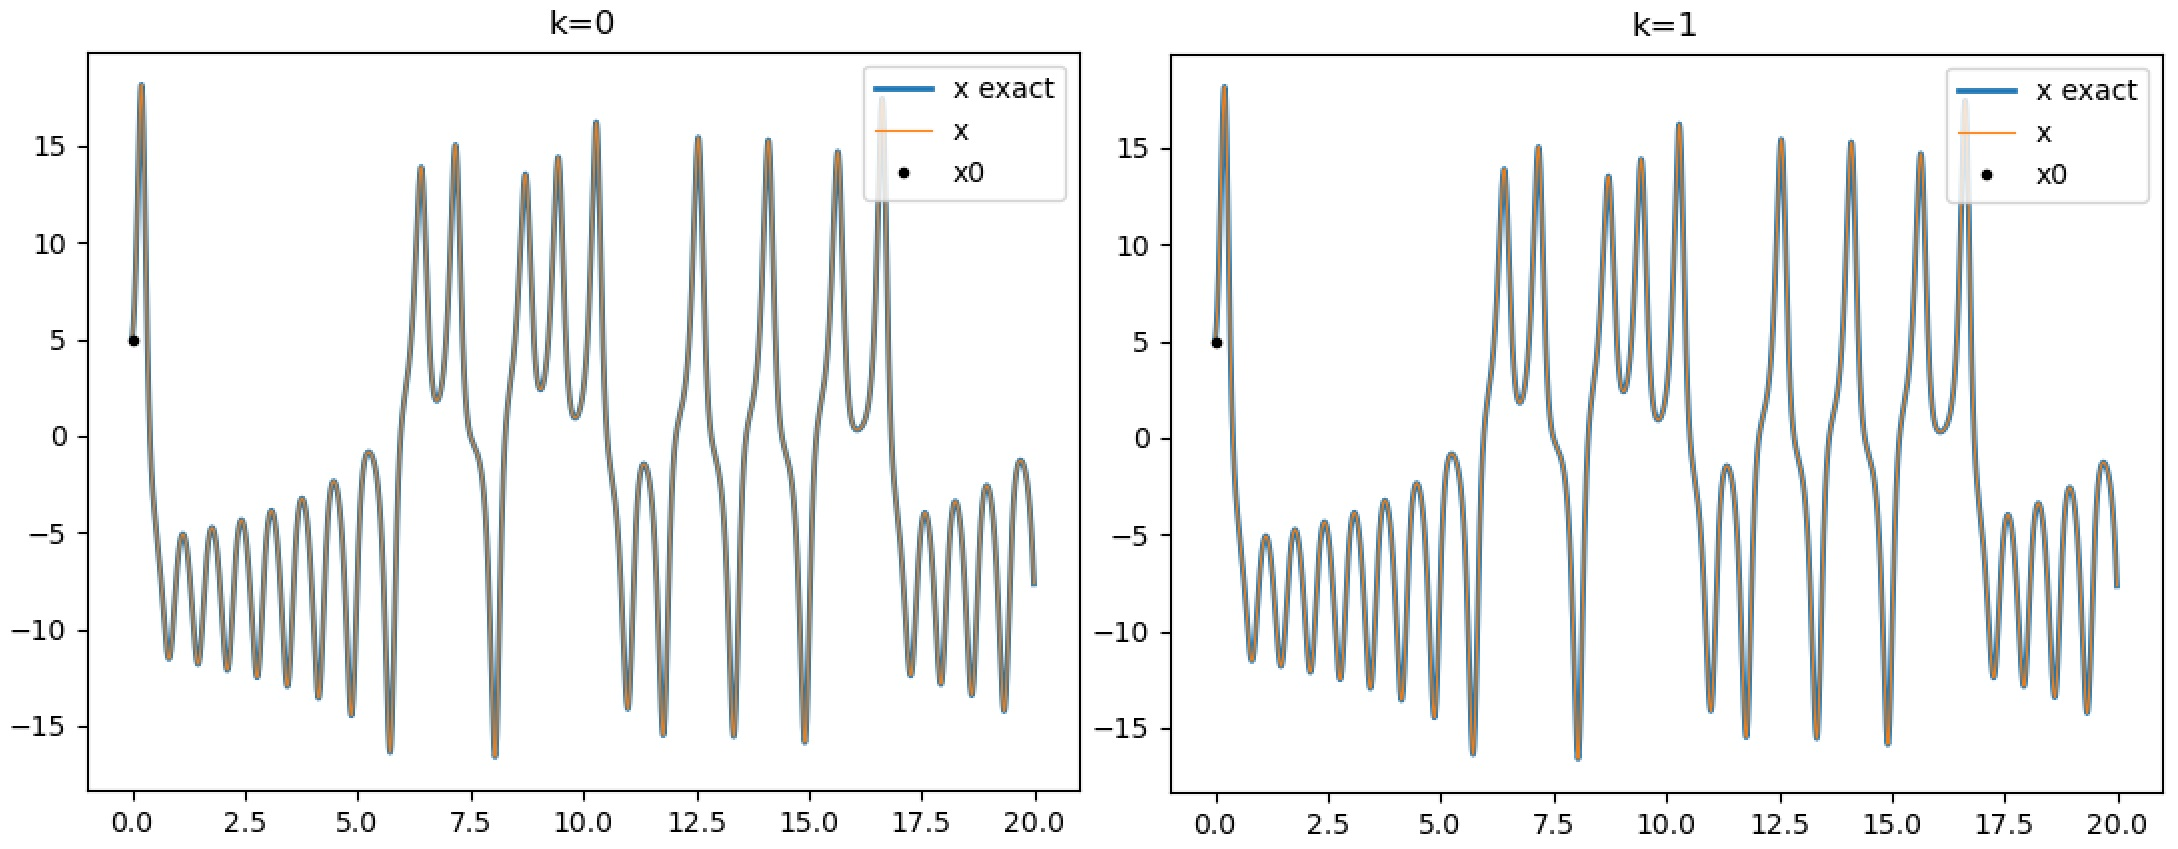
\includegraphics[width=0.55\linewidth]{"images/parareal/cpp/lorenz_1p.jpg"}
			\captionof{figure}{Parareal method on the Lorenz system with 1 process}
			\label{lorenz:1}
		\end{figure}
		\item With two processes we see that the solution converges in 2 iterations.
		\begin{figure}[H]      
			\qquad \qquad \qquad 
			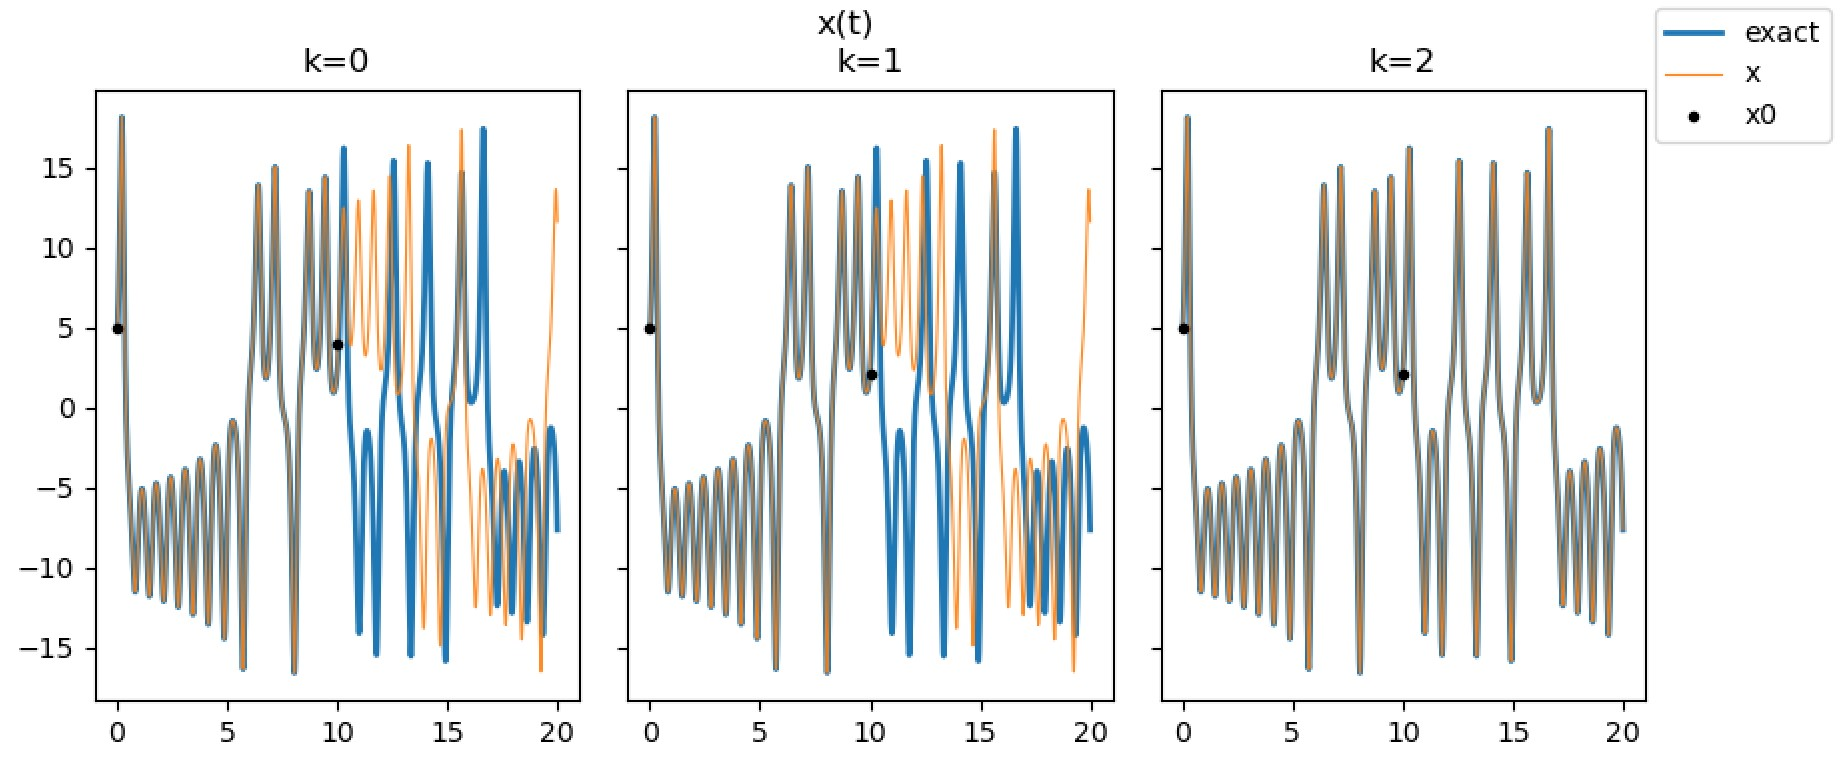
\includegraphics[width=0.8\linewidth]{"images/parareal/cpp/lorenz_2p.jpg"}
			\captionof{figure}{Parareal method on the Lorenz system with 2 processes}
			\label{lorenz:2}
		\end{figure}
		\item With three processes we see that the solution converges in 3 iterations.
		\begin{figure}[H] 
			\qquad \qquad \qquad       
			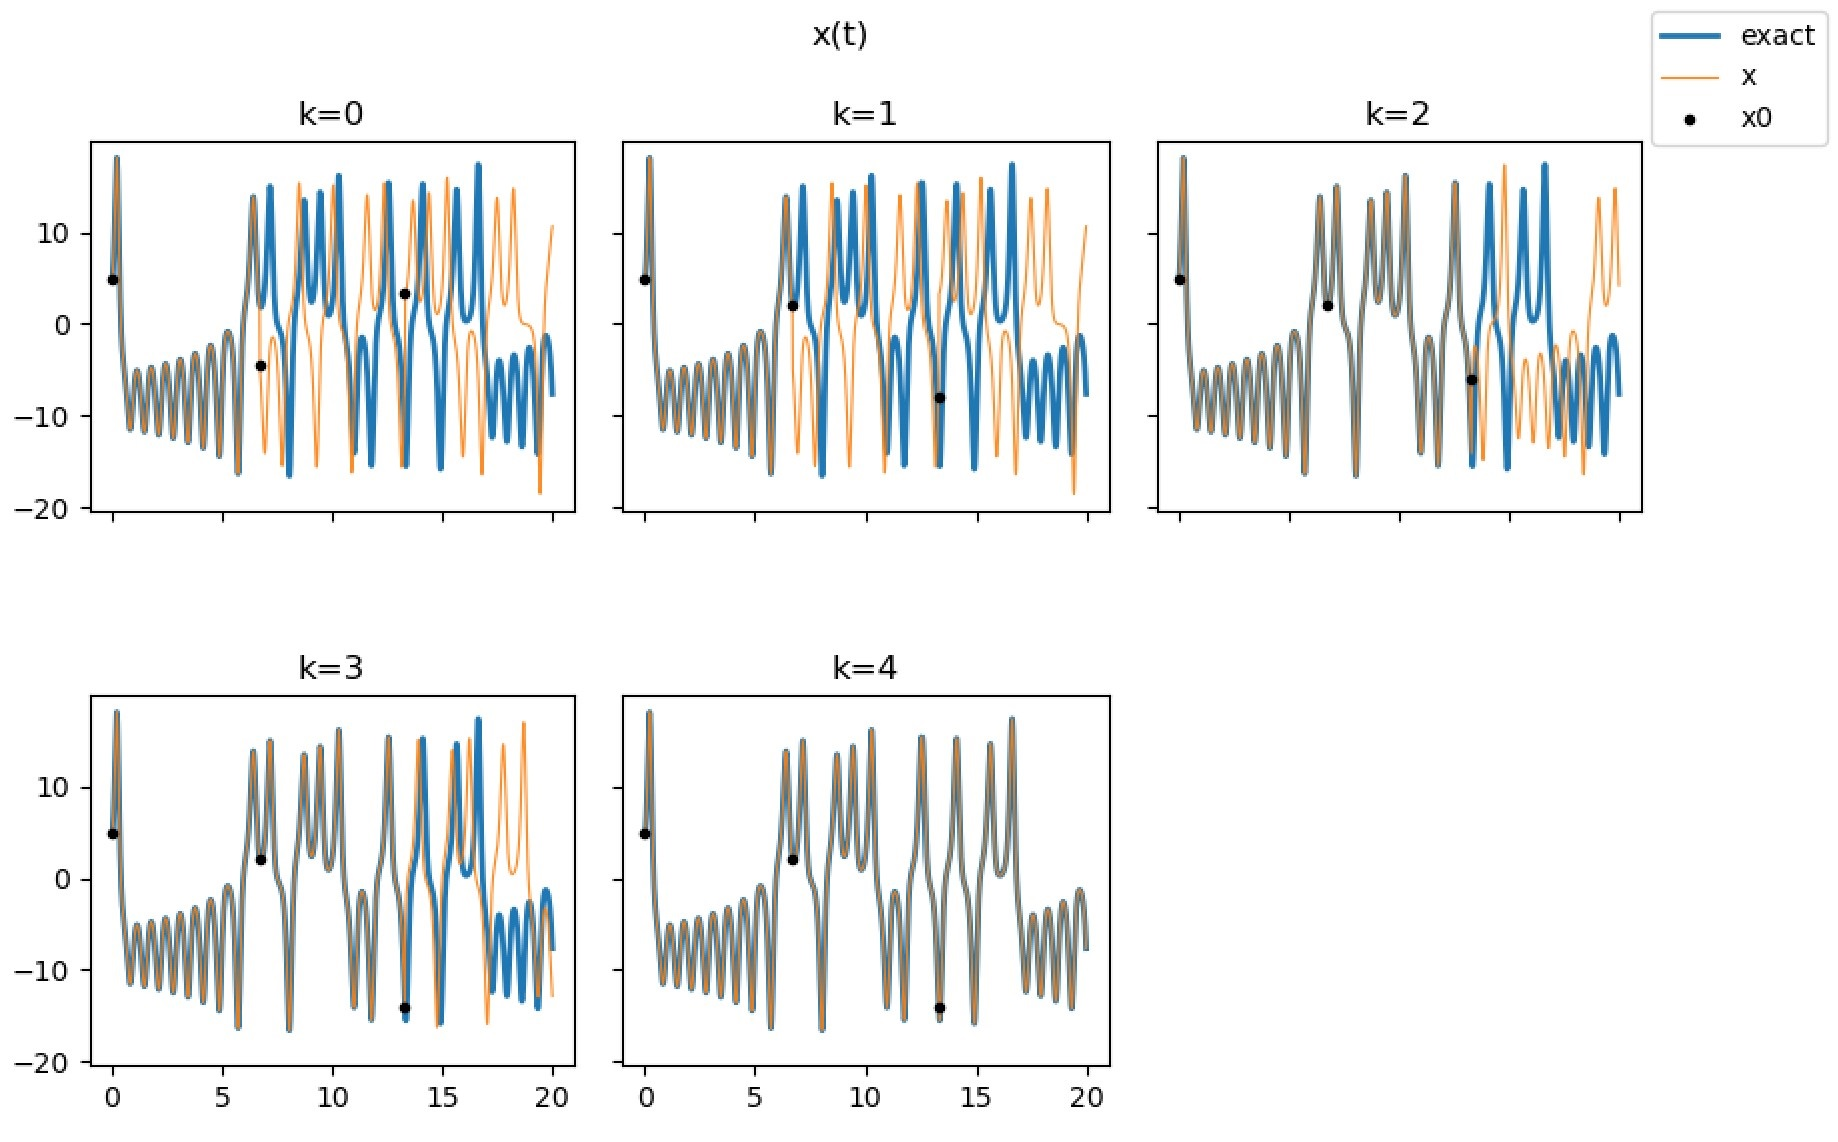
\includegraphics[width=0.45\linewidth]{"images/parareal/cpp/lorenz_3p.jpg"}
			\captionof{figure}{Parareal method on the Lorenz system with 3 processes}
			\label{lorenz:3}
		\end{figure}
		\newpage
		\item With four processes we see that the solution converges in 4 iterations.
		\begin{figure}[H]      
			\qquad \qquad
			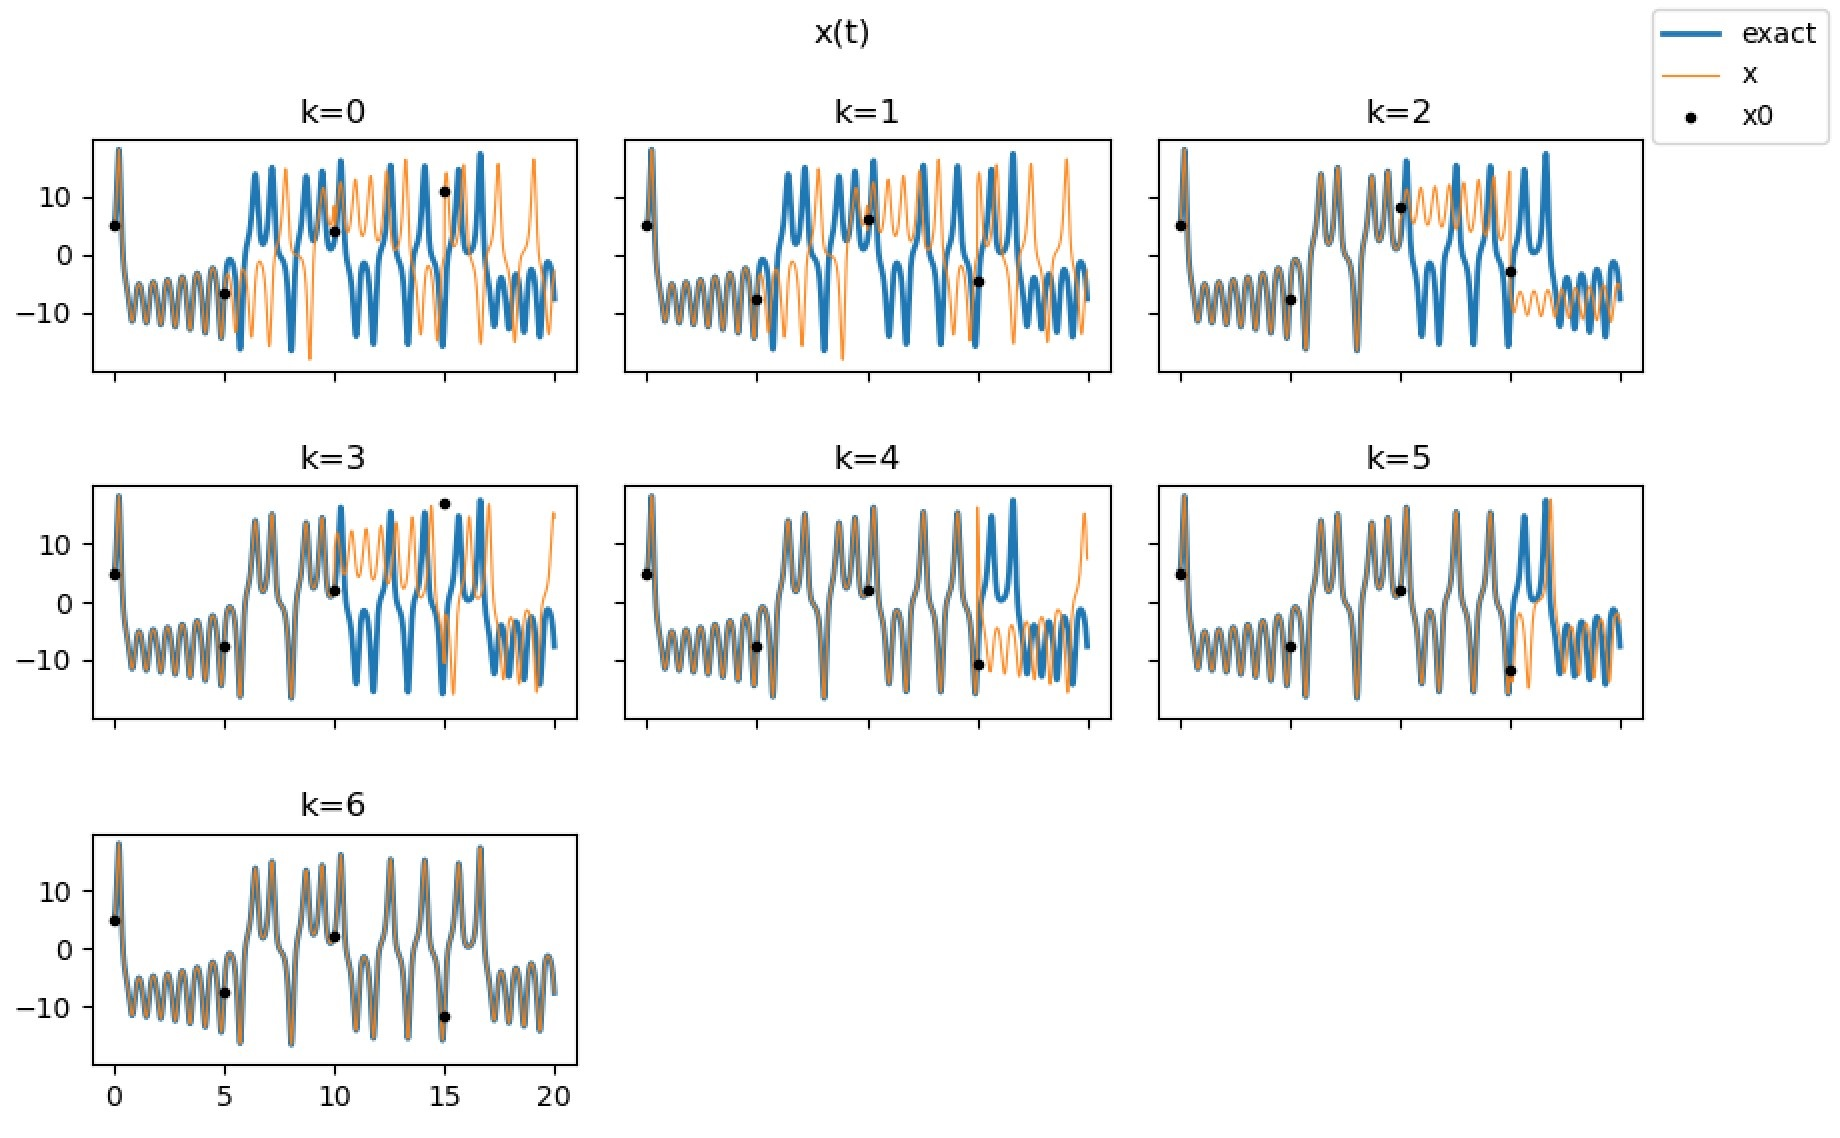
\includegraphics[width=0.7\linewidth]{"images/parareal/cpp/lorenz_4p.jpg"}
			\captionof{figure}{Parareal method on the Lorenz system with 4 processes}
			\label{lorenz:4}
		\end{figure}
	
	\end{enumerate}

\end{enumerate}

\subsubsection{Speed-up}
\label{speed_up}

The main objective of parallel methods is to reduce execution time by simultaneously performing tasks that can be done at the same time. In this section, we will study the speed-up achieved by the parareal method when the number of processes is increased. We will look at the speed-up with the Python implementation (done during the project) and the C++ implementation.

\begin{enumerate}[label=\textbullet]
	\item \textbf{Method implemented in Python :} \\
	The table below (Table \ref{time}) contains the execution time first of the iterative method with RK4 (the sequential method) and the execution time for different numbers of processes (parareal method) and this for various fine and coarse time steps by taking the following parameters for the Lorenz system :
	$$\sigma=10, \quad b=\frac{8}{3}, \quad r=28, \quad X_0=(5,5,5), \quad t_0=0, \quad T=200$$
	\renewcommand{\arraystretch}{1.2}
	\begin{table}[H]
		\centering
		\begin{tabular}{| c || c | c | c | c | c |}
			\hline
			\multirow{2}{1.5 cm}{$\Delta t$} & \multirow{2}{1.5 cm}{Seq} & \multirow{2}{1.5 cm}{1 proc} & \multirow{2}{1.5 cm}{2 proc} & \multirow{2}{1.5 cm}{3 proc} &\multirow{2}{1.5 cm}{4 proc} \\
			& & & & & \\
			\hline 
			F : 0.0025 & \multirow{2}{1.5 cm}{20s} & \multirow{2}{1.5 cm}{24s} & \multirow{2}{1.5 cm}{11s} & \multirow{2}{1.5 cm}{12s} & \multirow{2}{1.5 cm}{15s} \\
			G : 0.025 & & & & & \\
			\hline 
			F : 0.00125 & \multirow{2}{1.5 cm}{1m26} & \multirow{2}{1.5 cm}{1m40} & \multirow{2}{1.5 cm}{1m13} & \multirow{2}{1.5 cm}{47s} & \multirow{2}{1.5 cm}{52s} \\
			G : 0.0125 & & & & & \\
			\hline 
			F : 0.001 & \multirow{2}{1.5 cm}{1m44} & \multirow{2}{1.5 cm}{2m55} & \multirow{2}{1.5 cm}{1m26} & \multirow{2}{1.5 cm}{1m9} & \multirow{2}{1.5 cm}{1m24} \\
			G : 0.01 & & & & & \\	 
			\hline
		\end{tabular}
		\caption{Execution time with \textbf{Lorenz system} for various time steps in \textbf{Python}.}
		\label{time}
	\end{table}
	\newpage
	\noindent \underline{\textit{Observations :}} 
	\begin{itemize}[label=-]
		\item It seems that the time in sequential and with the parareal method with 1 process is not the same. Moreover for the different steps calculated, we have that the execution time with 1 process is greater than for the sequential method. This can be explained by 2 main things. First of all, we have seen previously that there are necessarily 2 iterations which are done on $[t_0,T]$ contrary to the sequential method where there is only one. This problem is easily solved if we compute only the fine and coarse solutions at the first iteration (because the point $U_0^k$ is identical for all k). Thereafter, the parareal method also computes the coarse solution which is not needed at all.
		\item It seems that the time for the parareal method with $P$ processes is not the time of the sequential method divided by $P$. It seems obvious that (with intervals of the same length for each process), the time for the parareal method is only divided by P if there is only one iteration, which is never the case.
		\item It seems that if we increase the number of processes, the time does not necessarily decrease (as between $P=3$ and $P=4$ for $\Delta t_F=0.001$ and $\Delta t_G=0.01$), so we have to find the right balance between the parameters $\Delta t_F$, $\Delta t_G$, $[t_0,T]$ and $P$.
	\end{itemize}
	\item \textbf{Method implemented in C++ :} \\
	First of all an interesting observation about the implementation of the parareal method in C++ is that it is much faster than Python (see Table \ref{cpp_faster}). \\
	For example let's take the following parameters for the Lorenz system :
	$$\sigma=10, \quad b=\frac{8}{3}, \quad r=28, \quad X_0=(5,5,5)$$
	$$t_0=0, \quad P=4,\quad \Delta t_G=0.01, \quad \Delta t_F=0.001$$
	Here are the execution times obtained in Python and C++ :
	\begin{table}[H]
		\centering
		\begin{tabular}{| c | c |}
			\hline
			Python : $T=200$ & C++ : $T=200000$ \\
			\hline 
			1m24s & 1m15s \\
			\hline
		\end{tabular}
		\caption{Difference of the execution times between Python and C++}
		\label{cpp_faster}
	\end{table}
	It can be seen that these times are of the same order as the problem in C++ is 1000 times larger than that in Python. This implies that to see a speed-up we must focus on much larger problems. For this we will take into account three parameters
	\begin{enumerate}[label=\textbullet]
		\item the size of the interval: $T$ (we will always take $t_0=0$)
		\item the precision of the fine time step : $\Delta t_F$
		\item the size of the problem to solve with the parareal method (in our case the Lorenz system)
	\end{enumerate}
	We will consider below two different problems :
	\begin{itemize}[label=-]
		\item \textbf{First problem : Harmonic oscillator.} (see Section ~\ref{oscillator_ode}) \\
		We will consider the harmonic oscillator with the following parameters :
		$$x(0) = 0, \quad v(0) = 1, \quad \omega_0 = 5, \quad x_0 = \frac{-1}{5}, \quad \phi_0 = \frac{\pi}{2}$$
		As the problem here is a rather small one we will increase its number of lines tenfold to be able to see a speed-up without having to take $T$ too large. In other words, instead of having 2 lines and thus 2 unknowns during the resolution we will have $2*d$ lines where $d$ is a chosen integer. \\
		For the parareal method, we will take the following parameters (where $T$ and $d$ will change):
		$$t_0=0, \quad T=\cdot, \quad \Delta t_G=0.01, \quad \Delta t_F=0.001, \quad d=\cdot$$
		\textbf{Example 1 :} We start by taking $T=10000$ and $d=100$, this is the execution times obtained :
		\renewcommand{\arraystretch}{1.2}
		\begin{table}[H]
			\centering
			\begin{tabular}{| c || c | c | c | c | c |}
				\hline
				\multirow{2}{1.5 cm}{$\cdot$} & \multirow{2}{1.5 cm}{Seq} & \multirow{2}{1.5 cm}{1 proc} & \multirow{2}{1.5 cm}{2 proc} & \multirow{2}{1.5 cm}{3 proc} &\multirow{2}{1.5 cm}{4 proc} \\
				& & & & & \\
				\hline 
				T : 10000 & \multirow{2}{1.5 cm}{17s} & \multirow{2}{1.5 cm}{36s} & \multirow{2}{1.5 cm}{30s} & \multirow{2}{1.5 cm}{29s} & \multirow{2}{1.5 cm}{24s} \\
				d : 100 & & & & & \\
				\hline 
			\end{tabular}
			\caption{Example 1 for the \textbf{harmonic oscillator}.}
			\label{time_osc_1}
		\end{table}
		It seems that when we apply the parareal method with only 1 process it is slower than with 2, 3 or 4 processes. However the time taken by the parareal method with 1 process is almost 2 times slower than with RK4 in sequential. However, the correct solution is obtained in all 5 cases:
		$$x(T)=-0.199968=\frac{-1}{5}\cos\left(5T+\frac{\pi}{2}\right)$$
		\textbf{Example 2 :} We will now double the number of equations ($d=200$) while keeping the same final time ($T=10000$) :
		\begin{table}[H]
			\centering
			\begin{tabular}{| c || c | c | c | c | c |}
				\hline
				\multirow{2}{1.5 cm}{$\cdot$} & \multirow{2}{1.5 cm}{Seq} & \multirow{2}{1.5 cm}{1 proc} & \multirow{2}{1.5 cm}{2 proc} & \multirow{2}{1.5 cm}{3 proc} &\multirow{2}{1.5 cm}{4 proc} \\
				& & & & & \\
				\hline 
				T : 10000 & \multirow{2}{1.5 cm}{28s} & \multirow{2}{1.5 cm}{59s} & \multirow{2}{1.5 cm}{49s} & \multirow{2}{1.5 cm}{48s} & \multirow{2}{1.5 cm}{41s} \\
				d : 200 & & & & & \\
				\hline 
			\end{tabular}
			\caption{Example 2 for the \textbf{harmonic oscillator}.}
			\label{time}
		\end{table}
		We make the same observation as before concerning the speed-up. However, we can see that by doubling the work to be provided by our methods, the execution times are not doubled. However, as in the previous example, we get the right solution in all 5 cases:
		$$x(T)=-0.199968=\frac{-1}{5}\cos\left(5T+\frac{\pi}{2}\right)$$
		\textbf{Example 3 :} Using the first example and doubling the final time ($T=20000$), we obtain :
		\begin{table}[H]
			\centering
			\begin{tabular}{| c || c | c | c | c | c |}
				\hline
				\multirow{2}{1.5 cm}{$\cdot$} & \multirow{2}{1.5 cm}{Seq} & \multirow{2}{1.5 cm}{1 proc} & \multirow{2}{1.5 cm}{2 proc} & \multirow{2}{1.5 cm}{3 proc} &\multirow{2}{1.5 cm}{4 proc} \\
				& & & & & \\
				\hline 
				T : 20000 & \multirow{2}{1.5 cm}{34s} & \multirow{2}{1.5 cm}{1m10s} & \multirow{2}{1.5 cm}{58s} & \multirow{2}{1.5 cm}{58s} & \multirow{2}{1.5 cm}{1m} \\
				d : 100 & & & & & \\
				\hline 
			\end{tabular}
			\caption{Example 3 for the \textbf{harmonic oscillator}.}
			\label{time_osc_3}
		\end{table}
		We can make the same observations as before and the solution obtained is correct:
		$$x(T)=0.00714986=\frac{-1}{5}\cos\left(5T+\frac{\pi}{2}\right)$$
		\underline{\textbf{Explanation :}} \\
		As explained in the examples it seems that the parareal method in C++ is not faster than the sequential version (with RK4) but on the contrary slower. This could be explained by the initialization which is in fact an additional iteration :
		\begin{figure}[H]      
			\qquad \qquad \qquad
			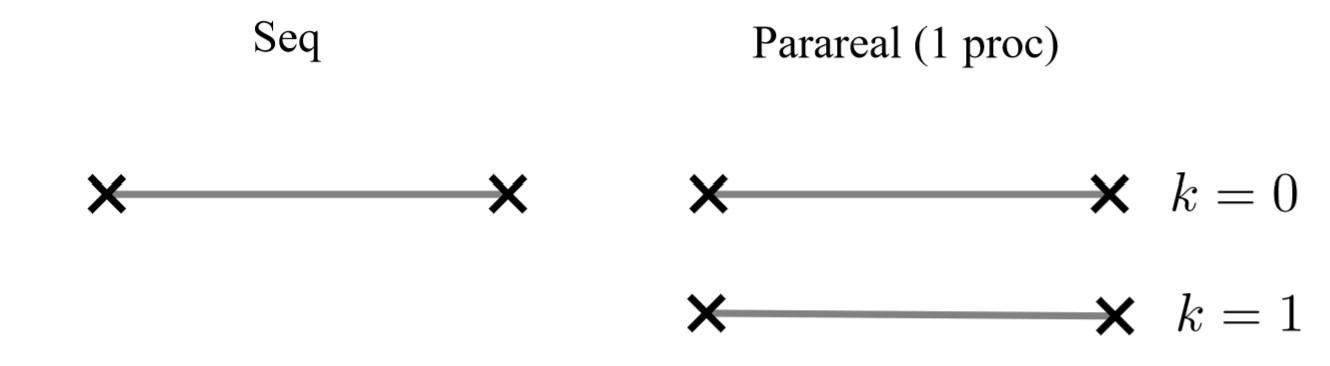
\includegraphics[width=0.7\linewidth]{"images/parareal/cpp/seq_vs_1proc.jpg"}
			\captionof{figure}{Explanation : Sequential vs Parareal with 1 process}
			\label{seq_vs_1proc}
		\end{figure}
		However, we can see that the parareal method with 2, 3 or 4 processes is faster than with a single process but still does not seem to be faster than the sequential method. Moreover as presented before there is a speed-up of the method with Python. \\
		For that we can make several hypothesis which will be presented in the Section \ref{improve}.
		\newpage
		\item \textbf{Second problem : Lorenz system.} (see Section ~\ref{lorenz_ode})
		We will now consider the Lorenz system with the following parameters :
		$$\sigma=10, \quad b=\frac{8}{3}, \quad r=28, \quad X_0=(5,5,5)$$
		As for the harmonic oscillator, the problem here is rather small, so we will increase the number of lines tenfold to be able to see an acceleration without having to take $T$ too large. In other words, instead of having 3 lines and thus 3 unknowns during the resolution, we will have $3*d$ lines where $d$ is a chosen integer. \\
		For the parareal method, we will take the following parameters (where $T$ and $d$ will change):
		$$t_0=0, \quad T=\cdot, \quad \Delta t_G=0.01, \quad \Delta t_F=0.001, \quad d=\cdot$$
		\textbf{Example 1 :} We start by taking $T=200$ and $d=10000$, this is the execution times obtained :
		\renewcommand{\arraystretch}{1.2}
		\begin{table}[H]
			\centering
			\begin{tabular}{| c || c | c | c | c | c |}
				\hline
				\multirow{2}{1.5 cm}{$\cdot$} & \multirow{2}{1.5 cm}{Seq} & \multirow{2}{1.5 cm}{1 proc} & \multirow{2}{1.5 cm}{2 proc} & \multirow{2}{1.5 cm}{3 proc} &\multirow{2}{1.5 cm}{4 proc} \\
				& & & & & \\
				\hline 
				T : 200 & \multirow{2}{1.5 cm}{53s} & \multirow{2}{1.5 cm}{1m46s} & \multirow{2}{1.5 cm}{1m29s} & \multirow{2}{1.5 cm}{1m25s} & \multirow{2}{1.5 cm}{1m27s} \\
				d : 10000 & & & & & \\
				\hline 
			\end{tabular}
			\caption{Example 1 for the \textbf{Lorenz system}.}
			\label{time_lorenz_1}
		\end{table}
		It seems as for the harmonic oscillator that when we apply the parareal method with only 1 process, it is slower than with 2, 3 or 4 processes. However the time taken by the parareal method with 1 process is almost 2 times slower than with RK4 in sequential. The results also seem to be correct in all cases since they are similar to those obtained by RK4 in sequential:
		$$(x(T),y(T),z(T))=(-5.65157, -1.7475, 28.839)$$
		\textbf{Example 2 :} We now divide by 2 the size of the problem ($d=5000$) while keeping the same $T=200$ :
		\begin{table}[H]
			\centering
			\begin{tabular}{| c || c | c | c | c | c |}
				\hline
				\multirow{2}{1.5 cm}{$\cdot$} & \multirow{2}{1.5 cm}{Seq} & \multirow{2}{1.5 cm}{1 proc} & \multirow{2}{1.5 cm}{2 proc} & \multirow{2}{1.5 cm}{3 proc} &\multirow{2}{1.5 cm}{4 proc} \\
				& & & & & \\
				\hline  
				T : 200 & \multirow{2}{1.5 cm}{25s} & \multirow{2}{1.5 cm}{53s} & \multirow{2}{1.5 cm}{44s} & \multirow{2}{1.5 cm}{42s} & \multirow{2}{1.5 cm}{44s} \\
				d : 5000 & & & & & \\
				\hline 
			\end{tabular}
			\caption{Example 2 for the \textbf{Lorenz system}.}
			\label{time_lorenz_2}
		\end{table}
		We can make the same observations as before but we notice this time that the size of the problem being divided by 2 the execution times are also divided by 2 in the 5 cases. We also obtain the same results:
		$$(x(T),y(T),z(T))=(-5.65157, -1.7475, 28.839)$$
		\textbf{Example 3 :} We will now look at a completely different case where we take a larger final time $T=500$ and fewer equations $d=1000$. Here are the execution times obtained:
		\begin{table}[H]
			\centering
			\begin{tabular}{| c || c | c | c | c | c |}
				\hline
				\multirow{2}{1.5 cm}{$\cdot$} & \multirow{2}{1.5 cm}{Seq} & \multirow{2}{1.5 cm}{1 proc} & \multirow{2}{1.5 cm}{2 proc} & \multirow{2}{1.5 cm}{3 proc} &\multirow{2}{1.5 cm}{4 proc} \\
				& & & & & \\
				\hline 
				T : 500 & \multirow{2}{1.5 cm}{13s} & \multirow{2}{1.5 cm}{27s} & \multirow{2}{1.5 cm}{22s} & \multirow{2}{1.5 cm}{23s} & \multirow{2}{1.5 cm}{22s} \\
				d : 1000 & & & & & \\
				\hline 
			\end{tabular}
			\caption{Example 3 for the \textbf{Lorenz system}.}
			\label{time_lorenz_3}
		\end{table}
		As far as execution times are concerned, there are not really any new observations to make. However, the results are different this time. Indeed, in the first 3 cases (sequential and  parareal with 1 and 2 processes) we obtain the same results:
		$$(x(T),y(T),z(T))=(-3.33169, -4.35437, 18.3289)$$
		But when we apply the parareal method with 3 or 4 processes we get completely different results. Below is what we get for 3 and 4 processes respectively:
		$$\text{3 proc : } (x(T),y(T),z(T))=(-0.935968, 0.240612,21.186)$$
		$$\text{4 proc : } (x(T),y(T),z(T))=(8.18609,1.32531,33.8032)$$
		Moreover we can observe that by keeping the same parameters as before but by refining the fine and coarse time steps the results change when using RK4 sequentially. We will take $\Delta t_F=0.0001$, this is what we obtain :
		$$(x(T),y(T),z(T))=(-0.46317,-2.72402,22.8864)$$
		\underline{\textbf{Explanation :}} \\
		To try to understand why we can obtain very different results by changing the number of parameters or the precision of the time steps, we have to look at the following new example: \\
		\textbf{Example 4 :} We will consider the Lorenz system with the following parameters :
		$$\sigma=10, \quad b=\frac{8}{3}, \quad r=28, \quad X_0=(5,5,5)$$
		$$t_0=0, \quad T=500, \quad \Delta t_G=0.1, \quad \Delta t_F=0.01, \quad d=1$$
		Here we are only interested in the use of parareal with 1 and 2 processes.
		\begin{enumerate}[label=\ding{213}]
			\item Applying the parareal method with 1 process, we obtain the results :
			$$(x(T),y(T),z(T))=(-9.63764,-14.9937,19.9616)$$
			These are the same results as with RK4 in sequential. \\
			By taking 2 processes for the parareal method, we obtain very different results:
			$$(x(T),y(T),z(T))=(-14.3485,-15.7886,33.3809)$$
			\item Using the \textit{diff} command of linux to compare 2 files, we realized that the difference that totally changes the final results of the method with 2 processes is a rounding to time $t=274,04s$. Indeed at this time, we have the following results with 1 and 2 processes :
			$$\text{1 proc : } (x,y,z)=( -13.0404,-9.45555,36.4169)$$
			$$\text{2 proc : } (x,y,z)=(-13.0405,-9.45558,36.4169)$$
			\item It is a very small difference but 10 seconds later, at time $t=284,04s$, the results are already starting to be less and less close:
			$$\text{1 proc : } (x,y,z)=( -0.102688,0.234586,16.7023)$$
			$$\text{2 proc : } (x,y,z)=(-0.043548,0.325784,16.7179)$$
			\item This small difference makes that 100 seconds later at $t=374,04s$, the results are not at all the same :
			$$\text{1 proc : } (x,y,z)=(13.0111,11.062,34.8919)$$
			$$\text{2 proc : } (x,y,z)=(-12.7836,-15.694,29.2703)$$
			\item This is how at time $T$, we obtain totally false results with 2 processes which is probably due to a rounding made at the initial time $t_1$ of this sub-interval. That is to say that $(x,y,z)(t_1)$ with 1 process is the right value but that $(x,y,z)(t_1)=U_1^1$ is wrongly computed, possibly because of the coarse integrator whose time step is not precise enough.
		\end{enumerate}
		Thus it seems that the more values to be calculated in the interval, the more errors can accumulate and therefore propagate to give false results. This is why the parareal method is perhaps not adapted to the Lorenz system due to the case theory (see section Ref) which makes that small errors can make the results diverge totally from the real solution.
	\end{itemize}
\end{enumerate}


\subsubsection{Efficiency}

The efficiency of a program in parallel allows to test the robustness of the code. By taking a problem of size $T$ and $P$ processes we obtain a certain execution time $t_e$. We will say that the problem is efficient if by taking a problem of size $2*T$ and $2*P$ processes the new execution time is in the range $[0.9t_e,1.1t_e]$. Here we will try to determine if the method implemented in C++ is efficient. Let's go back to Examples 1 and 3 of the harmonic oscillator in the Section \ref{speed_up}. So the parameters are as follows in the 2 examples:
$$x(0) = 0, \quad v(0) = 1, \quad \omega_0 = 5, \quad x_0 = \frac{-1}{5}, \quad \phi_0 = \frac{\pi}{2}$$
$$t_0=0, \quad T=\cdot, \quad \Delta t_G=0.01, \quad \Delta t_F=0.001, \quad d=100$$
In Example 1 we have $T=10000$ and in Example 3 we double the final time so $T=20000$, we then get the following execution times:
\renewcommand{\arraystretch}{1.2}
\begin{table}[H]
	\centering
	\begin{tabular}{| c || c | c |}
		\hline
		 & First case & Second case \\
		\hline
		Example 1 & Seq : 17s & \multirow{2}{2 cm}{2 proc : 30s}  \\
		$T=10000$ & 1 proc : 36s &  \\
		\hline 
		Example 2 & \multirow{2}{2 cm}{2 proc : 58s} & \multirow{2}{2 cm}{4 proc : 1m}  \\
		$T=20000$ & &  \\
		\hline 
	\end{tabular}
	\caption{Two tests of the efficiency of the parareal method in C++.}
	\label{efficiency}
\end{table}
\noindent It would seem that the method is not efficient and that doubling its size and the number of processes increases the execution time significantly. \\

\noindent \textbf{Explanation/Hypothesis :} \\
We will now try to understand why the method seems not to be efficient :
\begin{enumerate}[label=\textbullet]
	\item In the following, we will consider $t_0=0$. \\
	\textbf{First case :} We will try to understand why the method is not effective in the first case, here is a scheme: 
	\begin{figure}[H]      
		\centering
		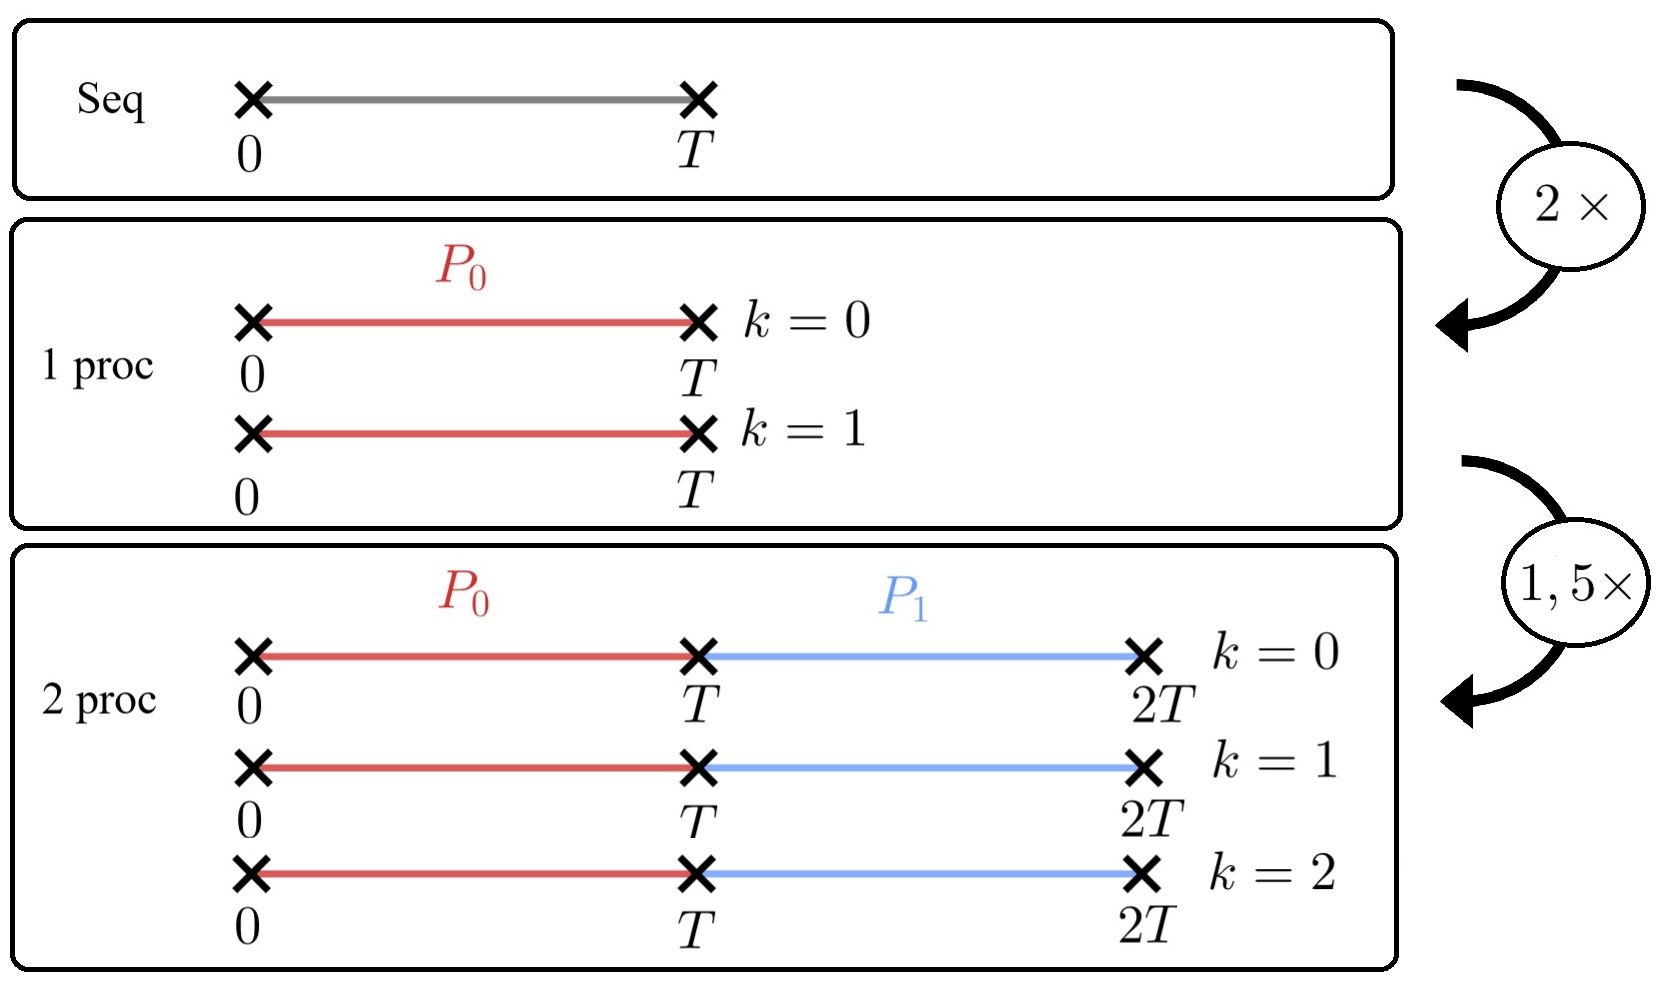
\includegraphics[width=0.5\linewidth]{"images/parareal/cpp/efficient_1_vs_2.jpg"}
		\captionof{figure}{Explanation : Sequential vs Parareal with 1 process}
		\label{efficient_1_vs_2}
	\end{figure}
	We see in the diagram above that RK4 in sequential solves the problem with the fine integrator between 0 and T, i.e. over $T$ seconds. \\
	The parareal method with 1 process performs the initialization ($k=0$) where it solves the problem with the fine integrator over $T$ seconds and performs a first iteration ($k=1$) where it solves the same problem once again : it therefore solves the problem over $2*T$ seconds and should therefore take twice as much time to execute as the sequential version. \\
	To check if the method is efficient, we want to solve the problem between 0 and $2T$ with 2 processes.  It solves three times the problem on $2*T$ with 2 processes (because 2 iterations and the initialization) thus $3*2*T$ seconds and each process solves the problem on $3*T$ seconds and thus it should take $1.5$ times more time than the parareal method with 1 process and $3$ times more time than in sequential.
	\textbf{Second case :} We will try now to understand why the method is not effective in the second case, here is a scheme: 
	\begin{figure}[H]      
		\qquad \qquad \qquad
		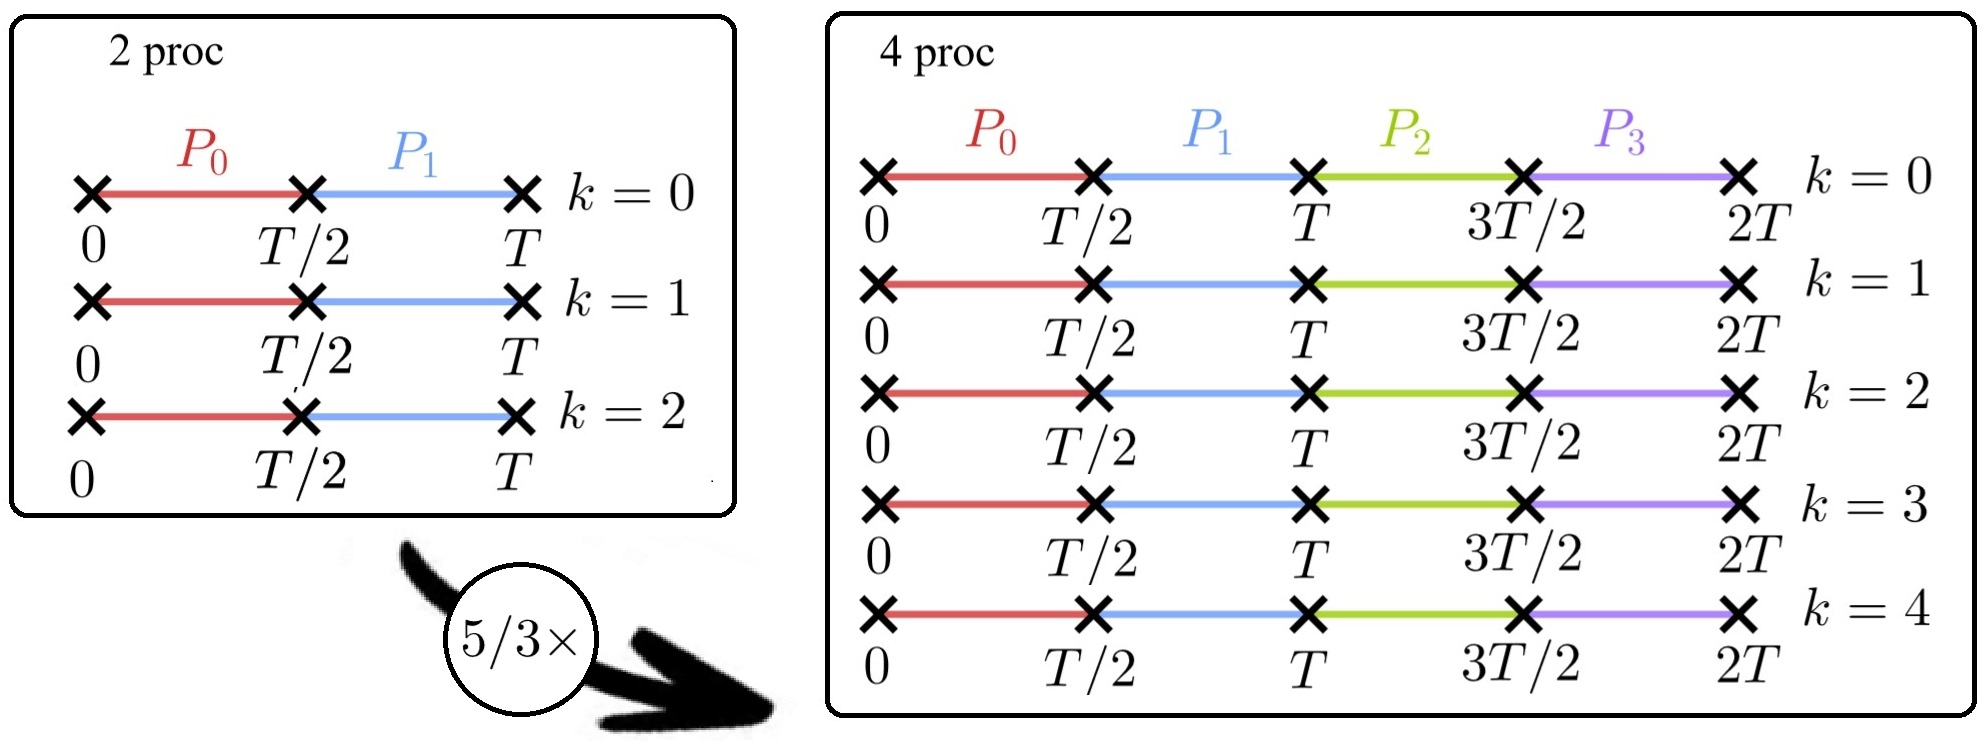
\includegraphics[width=0.7\linewidth]{"images/parareal/cpp/efficient_2p_vs_4p.jpg"}
		\captionof{figure}{Explanation : Sequential vs Parareal with 1 process}
		\label{efficient_2p_vs_4p}
	\end{figure}
	This time we want to solve the problem with the parareal method on 2 processes between 0 and $T$ or $T$ seconds. Each process solves the problem on $3*T/2$ seconds because of the 2 iterations and the initialization. \\
	To check if the method is efficient, we want to solve the problem on $2*T$ seconds with 4 processes. Each process then solves the problem on $T/2$ seconds 5 times because of the 4 iterations and the initialization thus $5*T/2$ seconds. So the parareal method with 4 processes should take $5/3$ times more time than the method with 2 processes.
	
	\item Then, it is also necessary to take into account that the method also uses the coarse integrator which must be used sequentially. These sequential parts also slow down the program and therefore the efficiency. Indeed if the fine integrator is used between 0 and $T$ and we double the size of the problem it will have to be computed between 0 and $2*T$ seconds, which will take 2 times more time. 
	
	\item One last point to take into account, even if it is smaller than the others, is that increasing the size of the problem also increases the number of operations and communications to do.
\end{enumerate}


\subsubsection{Order of the method}

\noindent Let us now check the order of convergenc (see Section \ref{order}) of the method on the harmonic oscillator with the following parameters :
$$x(0) = 0, \quad v(0) = 1, \quad \omega_0 = 5, \quad x_0 = \frac{-1}{5}, \quad \phi_0 = \frac{\pi}{2}$$
$$t_0=0, \quad T=200, \quad \Delta t_G=0.01, \quad \Delta t_F=0.001, \quad d=1$$
In the following graph, the blue curve represents the maximum on $j$ of $\mathcal{E}(j,k)$ according to the iterations $k$ and the orange curve represents the $(\Delta t_G)^k$.
\begin{figure}[H]
	\centering
	\fbox{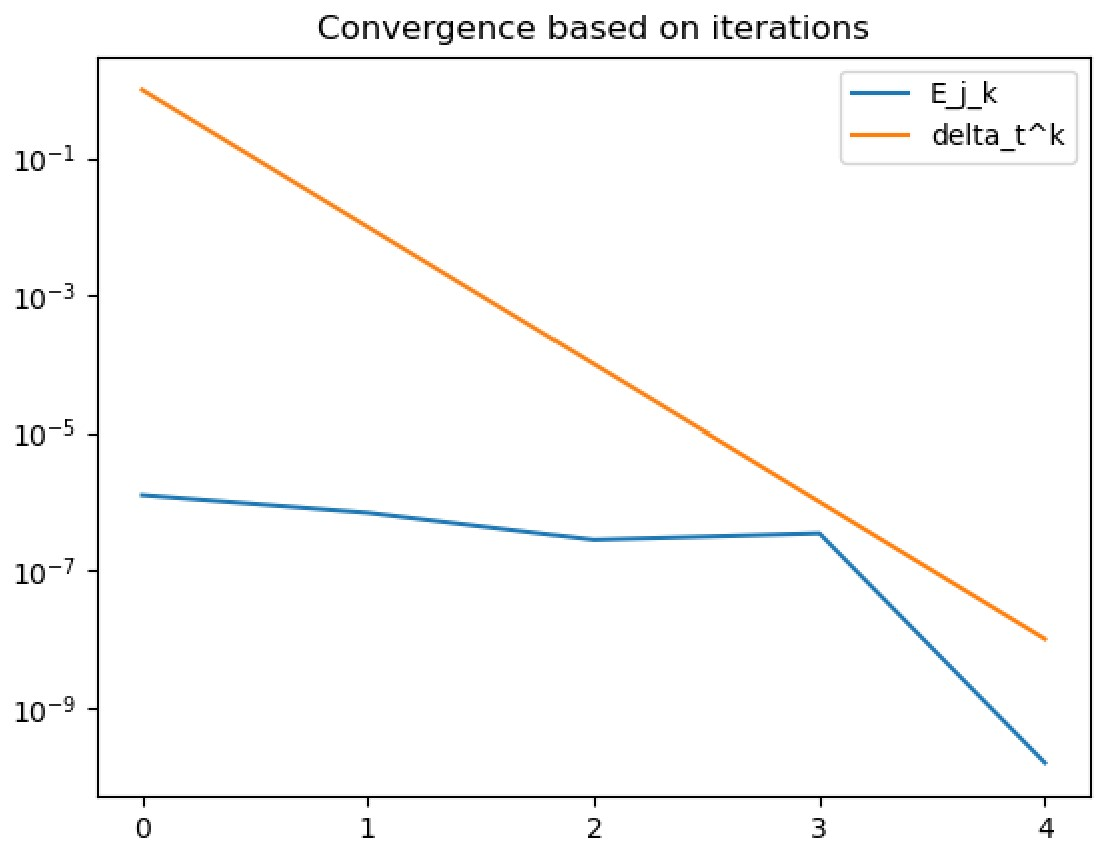
\includegraphics[width=0.3\linewidth]{"images/parareal/cpp/osci_cvg_1.jpg"}}
	\caption{Plot of $\mathcal{E}(j,k)$ and $(\Delta t_G)^k$ in \textbf{Python}.}
\end{figure}
\noindent We can see that the blue curve is below the orange curve for all the k iterations and so for the parameters fixed previously on the oscillator, the method is of order k.

\subsubsection{Conclusion for parareal method}
\label{improve}

\begin{itemize}[label=-]
	\item A first improvement for the implementation of the method could be to make a separate case for $P=1$. For this case, we would only compute the fine solution once on $[t_0,T]$.
	\item As said before, one possibility to improve the permorfances would be to compute only the fine and coarse solutions between $t_0$ and $t_1$ at the first iteration because they are the only ones that never change during the iterations. 
	\item In the same way, we could never compute the coarse solution between $t_{P-1}$ and $t_P$ because we never use it and we can compute the fine solution on this interval only at the last iteration (i.e. when the solution converges) because we need this information only to obtain the final solution of the system.
	\item We could see what happens if we take a lot more intervals that are spread over the different processes. Because here we are limited as the number of processes is equal to the number of intervals. Would we have an improvement for the speed of the method or on the contrary, would we have many more iterations because the initial points would be much less precise?
\end{itemize}


\subsection{Solving PDEs with Feel++}

\textbf{Goal :} Apply the parareal method to the resolution of the heat equation (see Section \ref{heat_pde}) using Feel++ which is a solver developed by Cemosis (see Section \ref{cemosis}) that uses the finite element method. \\
To solve the heat equation, we will use the finite element method which is a numerical method for solving PDE's and which is based on the approximation of the solution in the space $L^2/H^1$ which are spaces of infinite dimension. For these spaces there are bases of functions which will allow us to make a projection of the equations on these subspaces and to reduce the problem to find the solution to the projected equation which is the solution which minimizes the error among all the possible points of these subspaces. \\
Before starting to solve the heat equation by the parareal method using Feel++, we will first try to use Feel++ to solve the Laplace equation \cite{feelpp_laplacian}.

\subsubsection{Laplace equation}

\textbf{Explanation :} \\
We are interested in this section in the conforming finite element approximation of the Laplacian problem :
\begin{equation}
	\left\{\begin{aligned}
		-\Delta u &= f \quad&&\Omega \\
		u&=g \quad&&\Gamma_D \\
		\frac{\partial u}{\partial n} &=h \quad &&\Gamma_N \\
		\frac{\partial u}{\partial n}+u &=l \quad &&\Gamma_R \\
	\end{aligned}\right.
\end{equation}
We deduce the following weak formulation:
\begin{align*}
	-\int_\Omega \Delta u v &= \int_\Omega fv \\
	\int_\Omega \nabla u \cdot \nabla v - \int_{\partial\Omega}\frac{\partial u}{\partial n}v &= \int_\Omega fv \\
	\int_\Omega \nabla u \cdot \nabla v + \int_{\Gamma_R}uv &= \int_\Omega fv + \int_{\Gamma_N}hv+\int_{\Gamma_R}lv
\end{align*}
Thus we try to find $\; u:\Omega \mapsto \mathbb{R} \;$ such that $\; u\in H_{g,\Gamma_D}^1(\Omega) \;$ and
\begin{equation*}
	\int_\Omega \nabla u \cdot \nabla v + \int_{\Gamma_R}uv = \int_\Omega fv + \int_{\Gamma_N}hv+\int_{\Gamma_R}lv \quad \forall v\in H_{0,\Gamma_D}^1(\Omega)
\end{equation*}
i.e. find $\; u:\Omega \mapsto \mathbb{R} \;$ such that $\; u\in H_{g,\Gamma_D}^1(\Omega) \;$ and
\begin{equation*}
	a(u,v)=l(v)  \quad \forall v\in H_{0,\Gamma_D}^1(\Omega)
\end{equation*}
with
$$a(u,v)=\int_\Omega \nabla u \cdot \nabla v + \int_{\Gamma_R}uv, \quad l(v)=\int_\Omega fv + \int_{\Gamma_N}hv+\int_{\Gamma_R}lv$$
The Galerkin method is then used to determine the approximate variational problem. Let $(\varphi_i)$ a basis of $V_h$, this means $u_h(x)=\sum_{j=1}^{N_h}u_j\varphi_j(x)$ and then the approximate variationnel problem is written : \\
Find $\quad u_h\in V_h, \quad a(u_h,v_h)=l(v_h) \quad \forall v_h\in V_h$ \\
and then :
$$\begin{aligned}
	&a(u_h,v_h)=l(v_h) \\
	\iff &\sum_{j=1}^{N_h}u_ja(\varphi_j,v_h)=l(v_h) \quad &&\forall v_h\in V_h \\
	\iff &\sum_{j=1}^{N_h}u_ja(\varphi_j,\varphi_i)=l(\varphi_i) \quad &&\forall i\in\{1,\dots,N_h\} \\
	\iff &Au_h=b
\end{aligned}$$
with
$$A=(A_{i,j})_{i,j}=(a(\varphi_i,\varphi_j))_{i,j} \quad  \text{et} \quad b=(b_i)_i=(l(\varphi_i))_i$$

\noindent \textbf{Implementation with Feel++:} \\
We start by loading the mesh and defining all the elements we will need for the resolution. We can then define the bilinear form $a$ and the linear form $l$ of the variational formulation as well as the boundary conditions (Dirchlet, Neumann and Robin) by imposing by default Dirichlet conditions (see \cite{feelpp_laplacian}). \\

\noindent In the following we will consider the following geometry and the following mesh:
\begin{figure}[H]
	\begin{minipage}{0.48\linewidth}
		\centering
		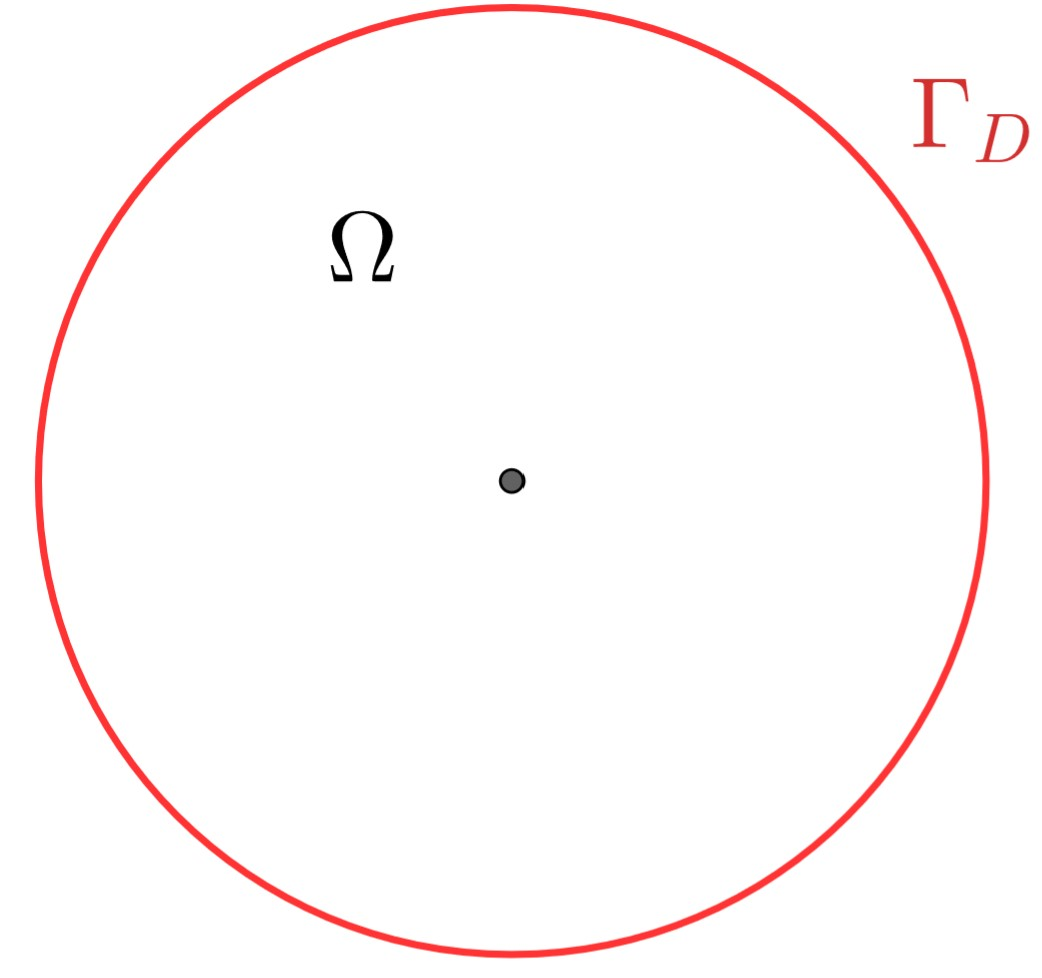
\includegraphics[width=0.7\linewidth]{"images/parareal/feelpp/circle.jpg"}
	\end{minipage}
	\begin{minipage}{0.48\linewidth}
		\centering
		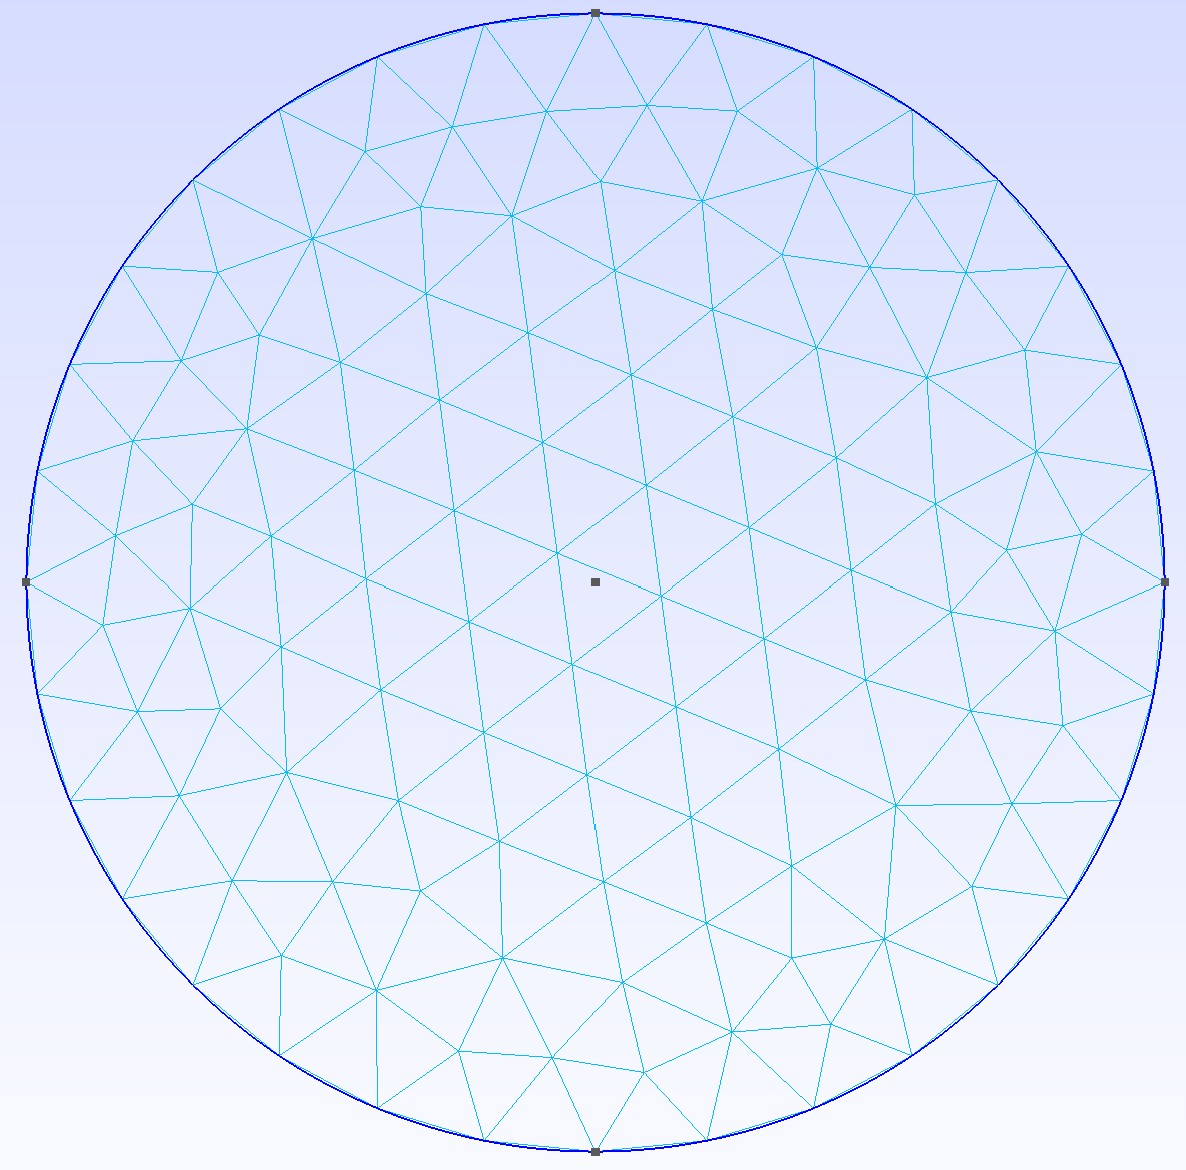
\includegraphics[width=0.7\linewidth]{"images/parareal/feelpp/circle_mesh.jpg"}
	\end{minipage}
	\caption{Geometry considered with its mesh (with Dirichlet)}
\end{figure}

\noindent\textbf{Example 1 :} \\
We consider :
$$\left\{\begin{aligned}
	-\Delta u &= f \quad&&\Omega \\
	u&=g \quad&&\Gamma_D \\
\end{aligned}\right. \quad \text{with} \quad
u_{exact}=g=x^2+y^2, \quad f=-\Delta u_{exact}=-4$$
\noindent We visualize the result with Paraview and we have the expected convergence results  with $P_{c,h}^1$:
$$||u-u_h||_{L^2}\sim h^2 \qquad \qquad ||u-u_h||_{H^1}\sim h^1$$
\begin{figure}[H]
	\begin{minipage}{0.48\linewidth}
		\centering
		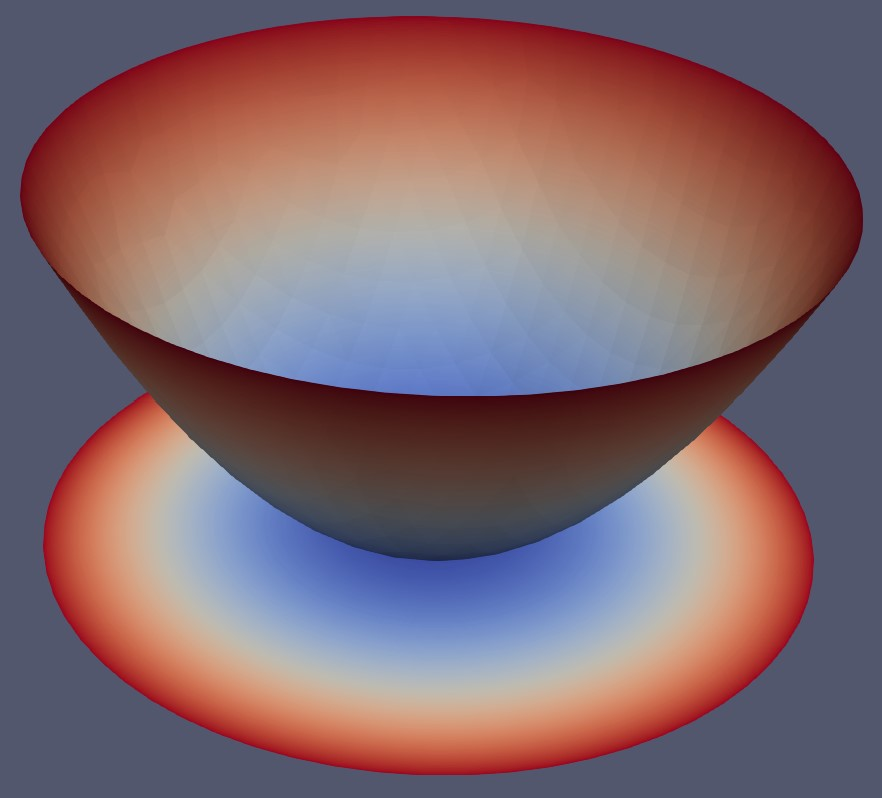
\includegraphics[width=0.8\linewidth]{"images/parareal/feelpp/circle_result.jpg"}
		\caption{Result (with Paraview)}
	\end{minipage}
	\begin{minipage}{0.48\linewidth}
		\centering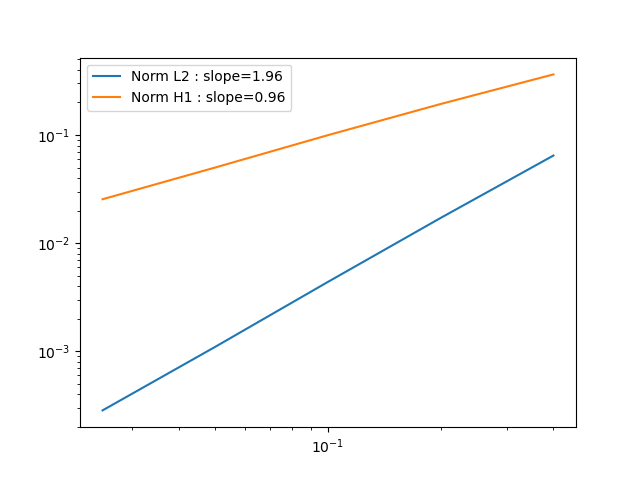
\includegraphics[width=0.9\linewidth]{"images/parareal/feelpp/cvg_laplacian_k1_o2.png"}
		\caption{Convergence order for the Laplacian problem with $P_{c,h}^1$.}
	\end{minipage}
\end{figure}

\noindent\textbf{Example 2 :} \\
We consider :
$$\left\{\begin{aligned}
	-\Delta u &= f \quad&&\Omega \\
	u&=g \quad&&\Gamma_D \\
\end{aligned}\right. \quad \text{with} \quad
u_{exact}=g=x^3+y^3, \quad f=-\Delta u_{exact}=-(6x+6y)$$
\noindent We visualize the result with Paraview and we have the expected convergence results  with $P_{c,h}^2$:
$$||u-u_h||_{L^2}\sim h^3 \qquad \qquad ||u-u_h||_{H^1}\sim h^2$$
\begin{figure}[H]
	\begin{minipage}{0.48\linewidth}
		\centering
		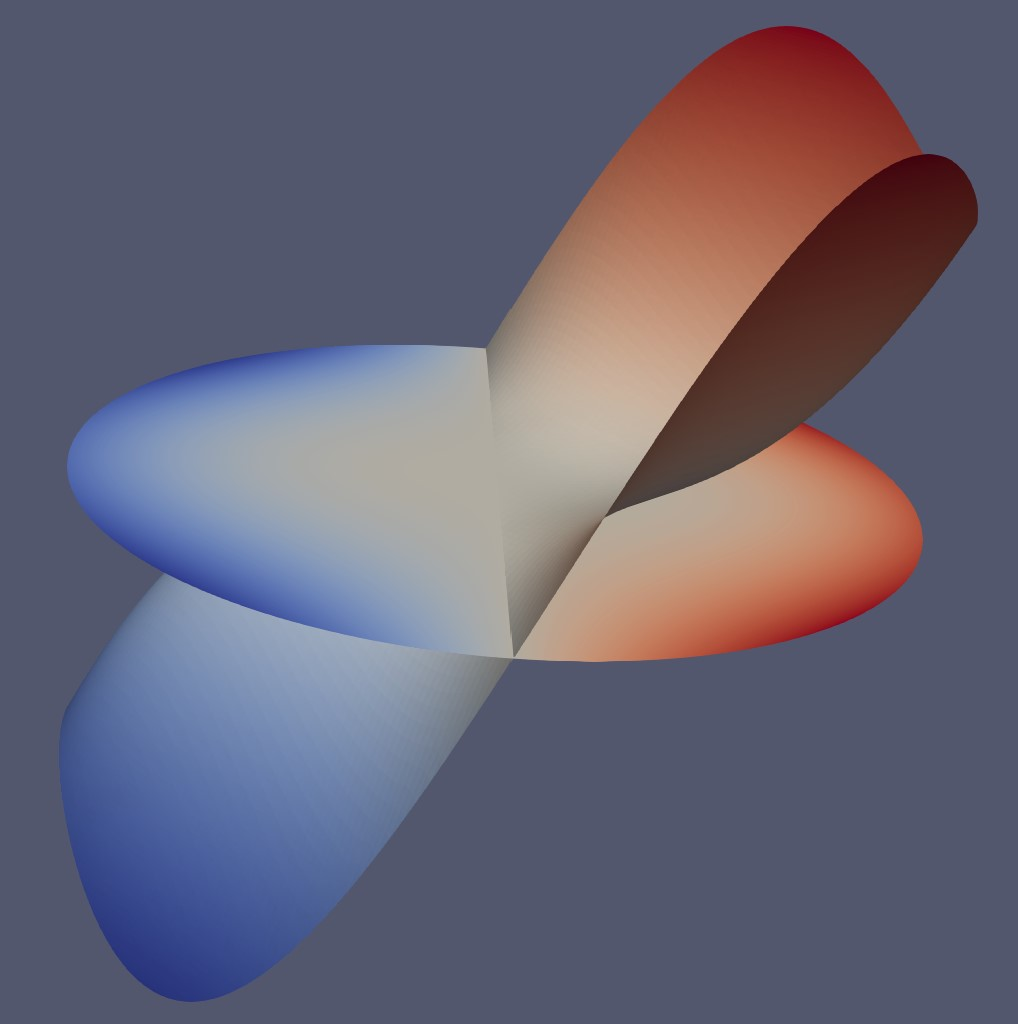
\includegraphics[width=0.7\linewidth]{"images/parareal/feelpp/circle_result_2.jpg"}
		\caption{Result (with Paraview)}
	\end{minipage}
	\begin{minipage}{0.48\linewidth}
		\centering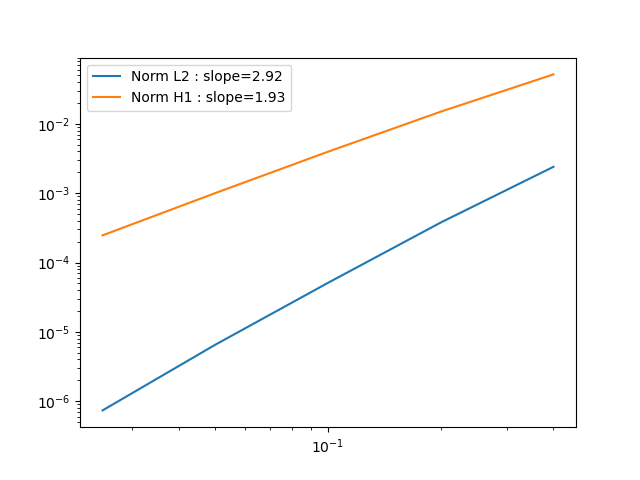
\includegraphics[width=0.9\linewidth]{"images/parareal/feelpp/cvg_laplacian_k2_o3.png"}
		\caption{Convergence order for the Laplacian problem with $P_{c,h}^2$.}
	\end{minipage}
\end{figure}

\noindent\textbf{Example 3 :} \\
We consider :
$$\left\{\begin{aligned}
	-\Delta u &= f \quad&&\Omega \\
	u&=g \quad&&\Gamma_D \\
\end{aligned}\right. \quad \text{with} \quad
u_{exact}=g=x^4+y^4, \quad f=-\Delta u_{exact}=-(12x^2+12y^2)$$
\noindent We visualize the result with Paraview and we have the expected convergence results  with $P_{c,h}^3$:
$$||u-u_h||_{L^2}\sim h^4 \qquad \qquad ||u-u_h||_{H^1}\sim h^3$$
\begin{figure}[H]
	\begin{minipage}{0.48\linewidth}
		\centering
		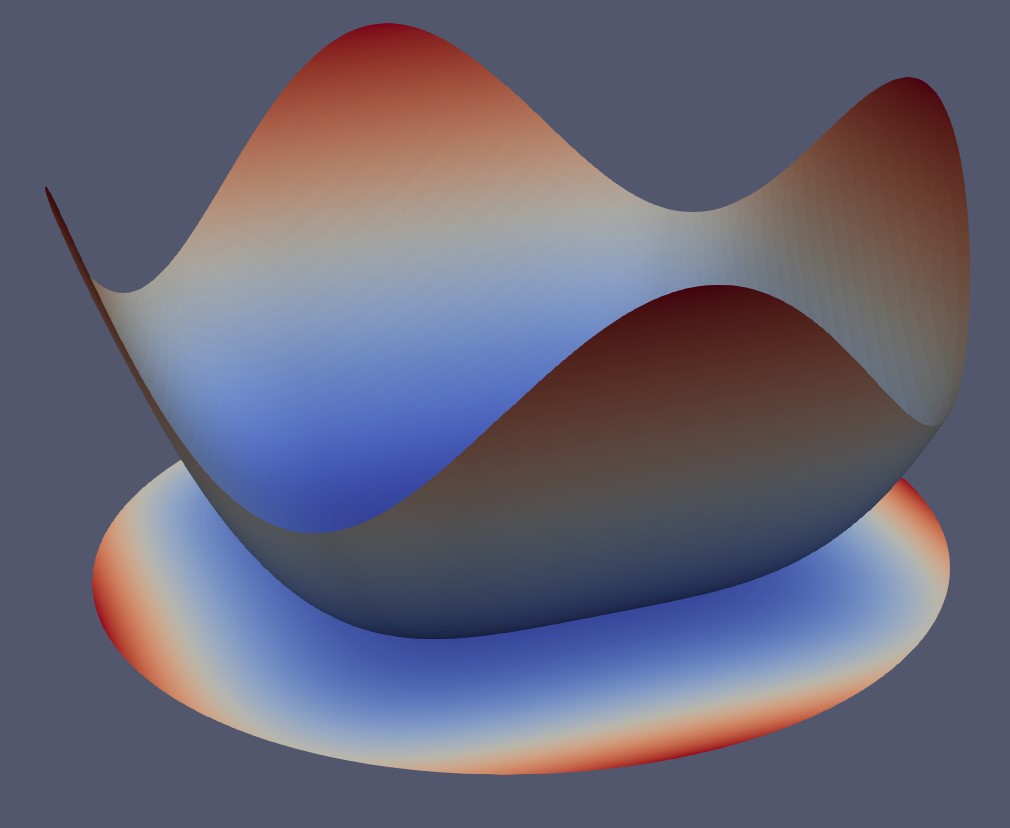
\includegraphics[width=0.7\linewidth]{"images/parareal/feelpp/circle_result_3.jpg"}
		\caption{Result (with Paraview)}
	\end{minipage}
	\begin{minipage}{0.48\linewidth}
		\centering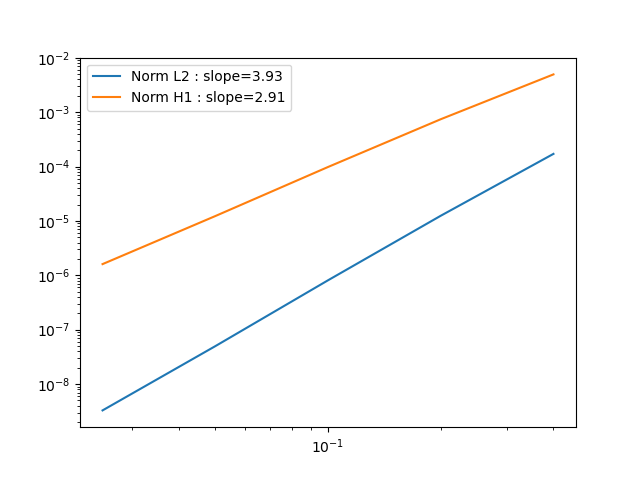
\includegraphics[width=0.9\linewidth]{"images/parareal/feelpp/cvg_laplacian_k3_o4.png"}
		\caption{Convergence order for the Laplacian problem with $P_{c,h}^3$.}
	\end{minipage}
\end{figure}